% !TeX spellcheck = en_US

\documentclass[12pt]{article}
\usepackage{colortbl}
\usepackage{tabularx}
\usepackage{longtable}
\usepackage{comment}
\usepackage{amsmath}
\usepackage{amssymb}
\usepackage{nccmath}
\usepackage{multirow}
%\usepackage{mathtools}
\usepackage{geometry}
\usepackage{booktabs}
\usepackage{xr}
\usepackage{enumitem}
\usepackage{siunitx}
\usepackage{graphicx}
\usepackage{pdflscape}
\usepackage{afterpage}
\usepackage{caption}
\usepackage{xr}
\usepackage{hyperref}
\usepackage[numbib,nottoc]{tocbibind}
\usepackage[round]{natbib}

\hypersetup{
    bookmarks=true,         % show bookmarks bar?
      colorlinks=true,       % false: boxed links; true: colored links
    linkcolor=red,          % color of internal links (change box
                            % color with linkbordercolor)
    citecolor=green,        % color of links to bibliography
    filecolor=magenta,      % color of file links
    urlcolor=cyan           % color of external links
}

%% Comments

\usepackage{color}

\newif\ifcomments\commentstrue

\ifcomments
\newcommand{\authornote}[3]{\textcolor{#1}{[#3 ---#2]}}
\newcommand{\todo}[1]{\textcolor{red}{[TODO: #1]}}
\else
\newcommand{\authornote}[3]{}
\newcommand{\todo}[1]{}
\fi

\newcommand{\wss}[1]{\authornote{blue}{SS}{#1}}
\newcommand{\an}[1]{\authornote{magenta}{Author}{#1}}


\newcommand{\progname}{SSP}

\newcommand{\colAwidth}{0.13\textwidth}
\newcommand{\colBwidth}{0.82\textwidth}
\newcommand{\colCwidth}{0.1\textwidth}
\newcommand{\colDwidth}{0.05\textwidth}
\newcommand{\colEwidth}{0.8\textwidth}
\newcommand{\colFwidth}{0.17\textwidth}
\newcommand{\colGwidth}{0.5\textwidth}
\newcommand{\colHwidth}{0.28\textwidth}
\newcounter{assumpnum} %Assumption Number
\newcommand{\atheassumpnum}{A\theassumpnum}
\newcommand{\aref}[1]{A\ref{#1}}
\newcounter{goalnum} %Goal Number
\newcommand{\gthegoalnum}{GS\thegoalnum}
\newcommand{\gsref}[1]{GS\ref{#1}}
\newcounter{theorynum} %Theory Number
\newcommand{\tthetheorynum}{T\thetheorynum}
\newcommand{\tref}[1]{T\ref{#1}}
\renewcommand{\arraystretch}{1}
\newcounter{instnum} %Instance Number
\newcommand{\itheinstnum}{IM\theinstnum}
\newcommand{\iref}[1]{IM\ref{#1}}
\newcounter{datadefnum} %Datadefinition Number
\newcommand{\ddthedatadefnum}{DD\thedatadefnum}
\newcommand{\ddref}[1]{DD\ref{#1}}
\newcounter{defnum} %Definition Number
\newcommand{\dthedefnum}{GD\thedefnum}
\newcommand{\dref}[1]{GD\ref{#1}}
\newcounter{reqnum} %Requirement Number
\newcommand{\rthereqnum}{R\thereqnum}
\newcommand{\rref}[1]{R\ref{#1}}
\newcounter{nfreqnum} %Non-functional Requirement Number
\newcommand{\nfrthenfreqnum}{NFR\thenfreqnum}
\newcommand{\nfrref}[1]{NFR\ref{#1}}
\newcounter{lcnum} %Likely change number
\newcommand{\lthelcnum}{LC\thelcnum}
\newcommand{\lcref}[1]{LC\ref{#1}}
\newcounter{ucnum} %Unlikely change number
\newcommand{\ltheucnum}{UC\theucnum}
\newcommand{\ucref}[1]{UC\ref{#1}}
\newcounter{tablenum} %Table number
\newcommand{\tablethetablenum}{Table\thetablenum}
\newcommand{\tableref}[1]{Table\ref{#1}}

\newcommand{\forceindent}{\parindent=1em\indent\parindent=0pt\relax}

%\oddsidemargin -1000mm
%\evensidemargin -1000mm
%\textwidth 160mm
%\textheight 300mm
\newgeometry{margin=2cm}

\externaldocument[MIS-]{MIS_SSP}
\externaldocument[MG-]{MG_SSP}

\begin{document}

\title{Software Requirements Specification for \progname: Slope Stability
  Analysis Program}
\author{Henry Frankis and Brooks MacLachlan}
\date{\today}
	
\maketitle

~\newpage

\pagenumbering{roman}

\section{Revision History}

\begin{tabularx}{\textwidth}{p{3cm}p{2cm}X}
	\toprule {\bf Date} & {\bf Version} & {\bf Notes}\\
	\midrule
	09/24/18 & 1.0 & Removed RFEM\\
	09/25/18 & 1.1 & Traceability matrix work\\
	09/26/18 & 1.2 & Physical System Description expanded, Non-functional 
	requirements itemized\\
	10/01/18 & 1.3 & Various improvements throughout\\
	10/02/18 & 1.4 & Initial revision of the solution characteristics 
	specification\\
	10/03/18 & 1.5 & Completed revision of the solution characteristics 
	specification and other sections\\
	10/04/18 & 1.6 & Minor fixes throughout\\
	10/12/18 & 1.7 & Minor fixes based on feedback\\
	10/17/18 & 1.8 & More fixes based on feedback\\
	12/05/18 & 1.9 & Completed major revisions\\
	\bottomrule
\end{tabularx}

~\newpage

\section{Reference Material} \label{sec_RefMat}
This section records information for easy reference.
\subsection{Table of Units}

The unit system used throughout is SI (Syst\`{e}me International d'Unit\'{e}s). 
In
 addition to the basic units, several derived units are also used. For each 
 unit, the table
 lists the symbol, a description and the SI name.
\newline

\renewcommand{\arraystretch}{1.2}
\setlength{\tabcolsep}{20pt}
\begin{tabular}{  l  l  l  }
\hline
\textbf{Symbol} & \textbf{Unit} & \textbf{SI} \\
\hline
\si{\newton} & force & newton \\
\si{\meter} & length & meter \\
$\si{\pascal}=\si{\newton\per\square\meter}$ & pressure & pascal \\
\si{\degree} & angle & degree  \\
\hline
\end{tabular}
\renewcommand{\arraystretch}{1}



\subsection{Table of Symbols}


The table that follows summarizes the symbols used in this document along with 
their units. 

\renewcommand{\arraystretch}{1.6}
\setlength{\tabcolsep}{20pt}
\begin{longtable*}{  l  l  p{8.5cm}  }
\hline
\textbf{Symbol} & \textbf{Unit} & \textbf{Description} \\
\hline
$A$ & \si{\meter\squared}& area on which a force acts
\\
$b$ & \si{\meter}& width of the base of a slice in the \textit{x}-direction
\\
\textit{const\_f} & & boolean decision on which form of \textit{f} 
the user desires: constant if true, or a half-sine if false
\\
$c'$ & \si{\pascal} & effective cohesion 
\\
${C_{\text{num},i}}$ & \si{\newton}& expression used to calculate the numerator 
of the interslice normal to shear force proportionality constant
\\
${C_{\text{den},i}}$ & \si{\newton}& expression used to calculate the 
denominator of the interslice normal to shear force proportionality constant
\\
$F$ & \si{\newton}& force
\\
${F_{x}}$ & \si{\newton} & $x$-component of force
\\
${F_{y}}$ & \si{\newton} & $y$-component of force
\\
$f$ & & variation of the interslice normal to shear force ratio as a function 
of distance in the $x$-direction
\\
$F_\text{S}$ & & factor of safety
\\
$F_\text{S}^{\text{Min}}$ & & minimum factor of safety associated with the 
critical slip surface
\\
$G$ & \si{\newton\per\meter} & interslice normal force per meter in the 
$z$-direction
\\
$H$ & \si{\newton\per\meter} & interslice water force per meter in the 
$z$-direction
\\
$h$ &  \si{\meter}& height in the \textit{y}-direction from the base of a slice 
to the slope surface, at the \textit{x}-direction midpoint of the slice
\\
$h_{\text{z}}$ & \si{\meter}& height in the \textit{y}-direction from the base 
of a slice to the center of the slice
\\
$h_\text{z,w}$ & \si{\meter}& height in the \textit{y}-direction from the base 
of a slice halfway to the water table
\\ 
$i$ & & index representing a single slice 
\\
${K_{\text{c}}}$ & & horizontal seismic coefficient
\\
$M$ & N \si{\meter}& moment
\\
$N$ & \si{\newton\per\meter} & normal force per meter in the $z$-direction
\\
$N'$ &\si{\newton\per\meter} & effective normal force per meter in the 
$z$-direction
\\
$n$ & & the total number of slices
\\
$P$ & \si{\newton\per\meter} & resistive shear force per meter in the 
$z$-direction
\\
$Q$ & \si{\newton\per\meter} & imposed surface load or external force per meter 
in the $z$-direction
\\
$R$ & \si{\newton\per\meter} & resistive shear force without the influence of 
interslice forces per meter in the $z$-direction
\\
$S$ & \si{\newton\per\meter} & mobilized shear force per meter in the 
$z$-direction
\\
$T$ & \si{\newton\per\meter} & mobilized shear force without the influence of 
interslice forces per meter in the $z$-direction
\\
${U_{\text{b}}}$ & \si{\newton\per\meter} & base hydrostatic force per meter in 
the $z$-direction
\\
${U_{\text{t}}}$ & \si{\newton\per\meter} & surface hydrostatic force per meter 
in the $z$-direction
\\
$u$ &\si{\pascal} & pore pressure from water within the soil
\\
$W$ & \si{\newton\per\meter} & self-weight per meter in the $z$-direction
\\
$X$ & \si{\newton\per\meter} & interslice shear force per meter in the 
$z$-direction
\\
$x$ & \si{\meter}& \textit{x}-ordinate in the Cartesian coordinate system
\\
$x_{\text{cs}}$ & \si{\meter} & \textit{x}-ordinate of a point on the critical 
slip 
surface
\\
${x_{\text{slip}}}$ &  \si{\meter}& \textit{x}-ordinate of a point on a slip 
surface
\\
${x_{\text{slip}}^{\text{maxExt}}}$ &  \si{\meter}& maximum potential 
\textit{x}-ordinate of 
the exit point of a slip surface
\\
${x_{\text{slip}}^{\text{maxEtr}}}$ &  \si{\meter}& maximum potential 
\textit{x}-ordinate 
of the entry point of a slip surface
\\
${x_{\text{slip}}^{\text{minExt}}}$ &  \si{\meter}& minimum potential 
\textit{x}-ordinate of 
the exit point of a slip surface
\\
${x_{\text{slip}}^{\text{minEtr}}}$ &  \si{\meter}& minimum potential 
\textit{x}-ordinate 
of the entry point of a slip surface
\\
${x_{\text{slope}}}$ &  \si{\meter}& \textit{x}-ordinate of a point on the slope
\\
${x_{\text{wt}}}$ & \si{\meter} & \textit{x}-ordinate of a point on the water 
table
\\
$y$ &  \si{\meter}& \textit{y}-ordinate in the Cartesian coordinate system
\\
$y_{\text{cs}}$ & \si{\meter} & \textit{y}-ordinate of a point on the critical 
slip 
surface
\\
${y_{\text{slip}}}$ & \si{\meter}& \textit{y}-ordinate of a point on a slip 
surface
\\
${y_{\text{slip}}^{\text{max}}}$ &  \si{\meter}& maximum potential 
\textit{y}-ordinate of a point on a slip surface
\\
${y_{\text{slip}}^{\text{min}}}$ &  \si{\meter}& minimum potential 
\textit{y}-ordinate of a point on a slip surface
\\
${y_{\text{slope}}}$ &  \si{\meter}& \textit{y}-ordinate of a point on the 
slope 
\\
${y_{\text{wt}}}$ &  \si{\meter}& \textit{y}-ordinate of a point on the water 
table
\\
$z$ & \si{\meter} & $z$-ordinate in the Cartesian coordinate system
\\
$\alpha{}$ & \si{\degree} & angle between the base of a slice and the horizontal
\\
$\beta{}$ &\si{\degree} & angle between the surface of a slice and the 
horizontal
\\
$\gamma{}$ & \si{\newton\per\cubic\meter} & soil dry unit weight
\\
${\gamma{}_{\text{Sat}}}$ &  \si{\newton\per\cubic\meter} & soil saturated unit 
weight
\\
${\gamma{}_{\text{w}}}$ & \si{\newton\per\cubic\meter} & unit weight of water
\\
$\lambda{}$ & & proportionality constant for the interslice normal to shear 
force ratio
\\
$\sigma{}$ & \si{\pascal} & total stress on the soil mass
\\
$\sigma{}_N'$ & \si{\pascal} & effective normal stress
\\
$\sigma{}'$ & \si{\pascal} & effective stress provided by the soil skeleton
\\
$\tau{}$ & \si{\pascal} & shear strength
\\
$\Upsilon{}$ & & generic minimization function or algorithm 
\\
$\varphi{}'$ & \si{\degree} & effective angle of friction
\\
$\Phi{}$ & & first function used to convert shear without the 
influence of interslice forces to shear with the influence of 
interslice forces
\\
$\Psi{}$ & & second function used to convert shear without the 
influence of interslice forces to shear with the influence of interslice 
forces
\\
$\omega{}$ & \si{\degree} & angle between the imposed surface load and the 
vertical
\\
${\ell{}_{\text{b}}}$ &  \si{\meter}& base length of a slice in the 
direction parallel to the slope of the base
\\
${\ell{}_{\text{s}}}$ &  \si{\meter}& surface length of a slice in the 
direction 
parallel to the slope of the surface \\

\hline
\end{longtable*}
\renewcommand{\arraystretch}{1}
\bmac{The two symbols $h_\text{z}$ and $h_\text{z,w}$ were originally $z$ and 
$z_w$. You commented "Why use z?". The reason is because they are z in the 
literature. However, since z is also used for coordinates, I changed these 
symbols and reserved z for coordinates}

\subsection{Abbreviations and Acronyms}

\renewcommand{\arraystretch}{1.2}
\begin{tabular}{l l} 
  \toprule		
  \textbf{Symbol} & \textbf{Description}\\
  \midrule 
  2D & Two-Dimensional\\
  A & Assumption\\
  DD & Data Definition\\
  GD & General Definition\\
  GS & Goal Statement\\
  IM & Instance Model\\
  LC & Likely Change\\
  NFR & Non-Functional Requirement\\
  PS & Physical System Description\\
  R & Requirement\\
  SRS & Software Requirements Specification\\
  \progname\ & Slope Stability analysis Program\\
  T & Theoretical Model\\
  TU & Typical Uncertainty\\
  UC & Unlikely Change\\
  \bottomrule
\end{tabular}\\

\newpage

\tableofcontents

~\newpage

\pagenumbering{arabic}

\setlength{\tabcolsep}{6pt}

\section{Introduction}

A slope of geological mass, composed of soil and rock and sometimes water, is 
subject to the influence of gravity on the mass. This can cause instability in 
the form of soil or rock movement. The effects of soil or rock movement can 
range from inconvenient to seriously hazardous, resulting in significant life 
and economic losses. Slope stability is of interest both when analysing natural 
slopes, and when designing an excavated slope. Slope stability analysis is the 
assessment of the safety of a slope, identifying the surface most likely to 
experience slip and an index of its relative stability known as the factor of 
safety.

~\newline
The following section provides an overview of the Software Requirements 
Specification (SRS) for a slope stability analysis problem. The developed 
program will be referred to as the Slope Stability analysis Program 
(\progname). This section explains the purpose of this document, the 
scope of the system, the characteristics of the intended readers, and the 
organization of the document.

\subsection{Purpose of Document}

The primary purpose of this document is to record the requirements of  
\progname{} and the models that will be used to meet those requirements. Goals, 
 assumptions,  theoretical models, definitions, and other model derivation 
 information are specified, allowing the reader to fully understand and verify 
 the purpose and scientific basis of \progname. With the exception of system 
 constraints in Section \ref{sec_SystConstraints}, this SRS will remain 
 abstract, describing \textit{what} problem is being solved, but not 
 \textit{how} to solve it.
~\newline

\noindent This document will be used as a starting point for subsequent 
development 
phases, including writing the design specification and the software verification
 and validation plan. The design document will show how the requirements
 are to be realized, including decisions on the numerical algorithms and 
programming environment. The verification and validation plan will show
 the steps that will be used to increase confidence in the software 
 documentation
 and the implementation. Although the SRS fits in a series of documents 
that follow the so-called waterfall model, the actual development process
 is not constrained in any way. Even when the waterfall model is not followed, 
as \cite{ParnasAndClements1986} point out, the most logical 
way to present the documentation is still to ``fake" a rational design process.

\subsection{Scope of Requirements} 

The scope of the requirements is stability analysis of a 2-Dimensional (2D)
soil mass, composed of a single homogeneous layer with constant material 
properties. The soil mass is assumed to extend infinitely in the third 
dimension. The analysis will be at an instant in time; factors that may change 
the slope properties over time will not be considered.

\subsection{Characteristics of Intended Reader}
\label{Sec:CharofInteRead}
Reviewers of this documentation should have an understanding of undergraduate 
Level 4 physics and should have completed a second year or higher level 
undergraduate course in solid mechanics. A course specifically in soil 
mechanics would be an asset. The users of \progname\ can have a 
lower level of expertise, as explained in Section~\ref{Sec:UserChar}.

\subsection{Organization of Document}

The organization of this document follows the template for an SRS for
scientific computing software proposed by~\cite{Koothoor2013} and
\cite{SmithAndLai2005}.  The presentation follows the standard pattern
of presenting goals, theories, definitions, and assumptions.  For
readers that would like a more bottom up approach, they can start
reading the instance models in Section \ref{sec_instance} and trace
back to find any additional information they require. The goal statements 
(Section \ref{sec_Goals}) are refined to the theoretical models, and the 
theoretical models (Section \ref{sec_theoretical}) to the instance models 
(Section \ref{sec_instance}). The instance models provide the set of algebraic 
equations that must be solved.

%\subsection{Intended Audience}

\section{General System Description}

This section provides general information about the system. It identifies the 
interfaces between the system and its environment, describes the user 
characteristics, and lists the system constraints.

\subsection{System Context}

Figure~\ref{Fig_SystemContext} shows the system context.  A circle represents an
external entity outside the software.  A rectangle represents the software 
system itself (\progname).  Arrows are used to show the data flow between the 
system and its environment.

\begin{figure}[h!]
	\begin{center}
		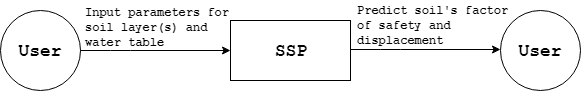
\includegraphics[width=0.8\textwidth]{SystemContextFigure.png}
		\caption{System Context}
		\label{Fig_SystemContext}
	\end{center}
\end{figure}

\noindent The responsibilities of the user and the system are as follows:

\begin{itemize}
\item User Responsibilities:
  \begin{itemize}
  \item Provide the input data related to the soil layer(s) and water table (if 
  applicable), ensuring conformation to input data format required by \progname
  \item Ensure that consistent units are used for input variables
  \item Ensure required software assumptions (Section~\ref{Assumptions}) are
    appropriate for the problem to which the user is applying the software
  \end{itemize}
\item \progname\ Responsibilities:
  \begin{itemize}
  \item Detect data type mismatch, such as a string of characters input instead
    of a floating point number
  \item Verify that the inputs satisfy the required physical constraints and 
  other data constraints (Section \ref{sec_DataConstraints})
  \item Identify the critical slip surface within the possible input range
  \item Find the factor of safety for the slope
  \item Find the interslice normal and shear forces along the critical slip 
  surface
  \end{itemize}
\end{itemize}

\subsection{User Characteristics}
\label{Sec:UserChar}
The end user of \progname\ should have an understanding of undergraduate
Level 1 Calculus and Physics, and be familiar with soil and material
properties, specifically cohesion, effective angle of friction, and unit weight.

\subsection{System Constraints} \label{sec_SystConstraints}

The Morgenstern-Price method \citep{MorgPrice}, which involves dividing the 
slope into vertical 
slices, will be used to derive the equations for analysing the slope. 

\section{Specific System Description}

This section first presents the problem description, which gives a
high-level view of the problem to be solved.  This is followed by the
solution characteristics specification, which presents the
assumptions, theories, definitions and finally the instance models.

\subsection{Problem Description} \label{Sec_pd}

\progname\ is a computer program developed to evaluate the factors of safety 
for a slope's slip surfaces and identify the critical slip surface of the 
slope, as well as the interslice normal and shear forces along the critical 
slip surface. It is intended to be used as an educational tool for introducing 
slope stability issues, and to facilitate the analysis and design of a safe 
slope.

\subsubsection{Terminology and Definitions}

This subsection provides a list of terms that are used in the subsequent
sections and their meaning, with the purpose of reducing ambiguity and
 making it easier to correctly understand the requirements.

\begin{itemize}
\item {\textit{Factor of safety:} The global stability metric of a slip surface 
of a slope, defined as the ratio of resistive shear force to mobile shear force}
  
\item {\textit{Slip surface:} A surface within a slope that has the potential 
to fail or displace due to load or other forces.}

\item {\textit{Critical slip surface:} Slip surface of the slope that
  has the lowest factor of safety, and is therefore most likely to
  experience failure.}

\item {\textit{Water table:} The upper boundary of a saturated zone in the 
ground.}

\item {\textit{Stress:} Force applied over an area.}
  
\item {\textit{Strain:} A measure of deformation of a body or plane under 
stress.}
  
\item {\textit{Normal force:} A force applied perpendicular to the
  plane of the material.}
  
\item {\textit{Shear force:} A force applied parallel to the plane of
  the material.}

\item {\textit{Resistive shear force:} Shear force in the direction opposite to 
the direction of potential motion, thus hindering motion along the plane.}
	
\item {\textit{Mobile shear force:} Shear force in the direction of potential 
motion, thus encouraging motion along the plane.}

\item{\textit{Effective forces and stresses}: The normal force or stress 
carried by the soil skeleton. The total normal force or stress is composed of 
the effective force or stress and the force or stress exerted by water.}
	
\item {\textit{Cohesion:} An attractive force between adjacent particles that 
holds the matter together.}
  
\item {\textit{Isotropic:} A condition where the value of a property is 
independent of the direction in which it is measured.}
  
\item {\textit{Plane strain:} A condition where the resultant stresses in one 
of the directions of a 3-dimensional body can be approximated as
  zero. Results when the length of one dimension of the body dominates
  the others, to the point where it can be assumed as infinite. Stresses in the 
  direction of the dominant dimension can be approximated as zero.}

\end{itemize}

\subsubsection{Physical System Description} \label{sec_system}

The Physical System (PS) of \progname{}, as shown in Figure~\ref{Fig_PhysSyst}, 
includes the following elements:

\begin{itemize}
\item[PS1:] A slope comprised of one layer of soil.
\item[PS2:] A water table, which may or may not exist.
\end{itemize}

\begin{figure}[h!]
	\begin{center}
		{
			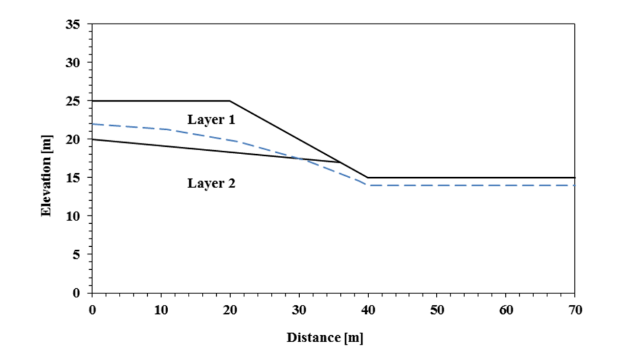
\includegraphics[width=0.7\textwidth]{PhysSyst.png}
		}
		\caption{An example slope for analysis by \progname{}, where the dashed 
		line represents the water table}
		\label{Fig_PhysSyst}
	\end{center}
\end{figure}

~\newline\noindent Morgenstern-Price \citep{MorgPrice} analysis of the slope 
involves representing the slope as a series of vertical slices. As shown in 
Figure~\ref{Fig_Index}, the index $i$ is used to denote a value for a single 
slice, and an interslice value at a given index $i$ refers to the value between 
slice $i$ and adjacent slice $\textit{i}+1$.

\begin{figure}[h!]
\begin{center}
{
\setlength{\unitlength}{6cm}
\begin{picture}(2,1)
% BORDER %
\thinlines
\put(0,0){\line(0,1){1}}
\put(0,1){\line(1,0){2}}
\put(2,1){\line(0,-1){1}}
\put(2,0){\line(-1,0){2}}
% SLIP SURFACE %
\linethickness{1mm}
\qbezier(0.2, 0.9)(0.5, 0.3)(1.8, 0.1)
% SLOPE %
\linethickness{0.1mm}
\put(0.1,0.9){\line(1,0){0.5}}
\put(0.6,0.9){\line(3,-2){1.2}}
\put(1.8,0.1){\line(1,0){0.1}}
% SLICES %
\put(0.2,0.9){\line(0,1){0}}
\put(0.6,0.484){\line(0,1){0.416}}
\put(0.9,0.33){\line(0,1){0.368}}
\put(1.05,0.27){\line(0,1){0.333}}
\put(1.4005,0.1764){\line(0,1){0.19}}
\put(1.8,0.1){\line(0,1){0}}
% interslice LABELS %
\put(0.55,0.92){$i=1$}
\put(0.85,0.75){$i=2$}
\put(1.05,0.65){$i=n-2$}
\put(1.3985,0.3863){$i=n-1$}
% slice LABELS %
\put(0.38,0.75){$i=1$}
\put(0.7,0.6){$i=2$}
\put(0.93,0.45){$\dots$}
\put(1.1,0.3){$i=n-1$}
\put(1.48,0.185){$i=n$}
\end{picture}
}
\caption{Index convention for slice and interslice values}
\label{Fig_Index}
 \end{center}
\end{figure}


\noindent A free body diagram of the forces acting on a slice is displayed in 
Figure~\ref{Fig_Forces}. The specific forces and symbols will be discussed in 
detail in Sections~\ref{sec_gendef} and \ref{sec_datadef}.

\begin{figure}[h!]
\begin{center}
{
 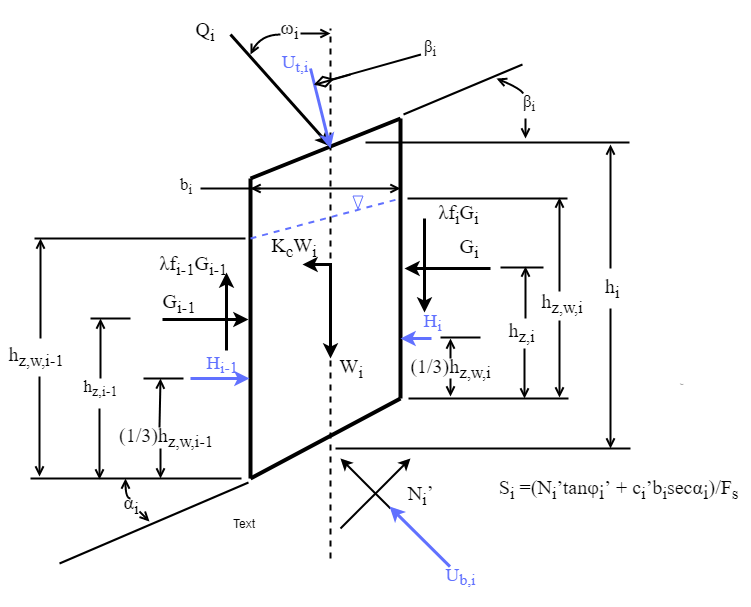
\includegraphics[width=0.7\textwidth]{ForceDiagram.png}
}
\caption{Free body diagram of forces acting on a slice}
\label{Fig_Forces}
\end{center}
\end{figure}

\subsubsection{Goal statements} \label{sec_Goals}

Given the shape of a soil mass, the location of a water table, and the material 
properties of the soil, the goal statements are to:

\begin{itemize}
\item [GS\refstepcounter{goalnum}\thegoalnum: \label{G_Critical}]
  {Identify the critical slip surface and the corresponding factor of safety.}

\item [GS\refstepcounter{goalnum}\thegoalnum: \label{G_Normal}]
  {Determine the interslice normal force between each pair of vertical slices   
  of the slope.}
  
\item [GS\refstepcounter{goalnum}\thegoalnum: \label{G_Shear}]
  {Determine the interslice shear force between each pair of vertical slices of 
  the slope.} 
\end{itemize}

\subsection{Solution Characteristics Specification}

The instance models that govern \progname\ are presented in
Section~\ref{sec_instance}.  The information to understand the
meaning of the instance models and their derivation is also presented,
so that the instance models can be verified.

\subsubsection{Assumptions}
\label{Assumptions}
This section simplifies the original problem and helps in developing the
theoretical models by filling in the missing information for the physical
system. The numbers given in the square brackets refer to the theoretical model
[T], general definition [GD], data definition [DD], instance model [IM], or
likely change [LC], in which the respective assumption is used.

\begin{enumerate}[label=A\arabic*:,ref={\arabic*}]
\item [A\refstepcounter{assumpnum}\theassumpnum: \label{A_Concave}] The
  slip surface is concave with respect to the slope surface. The 
  $(x_{\text{slip}},y_{\text{slip}})$ coordinates of a slip surface follow a 
  concave up 
  function. [\iref{IM_Min}]

\item [A\refstepcounter{assumpnum}\theassumpnum: \label{A_Constant}] The factor 
of safety is assumed to be constant across the entire slip surface. 
[\dref{GD_MobShear}]

\item [A\refstepcounter{assumpnum}\theassumpnum: \label{A_Homo}] The soil mass 
is homogeneous, with consistent soil properties throughout. [\dref{GD_P}, 
\ddref{DD_W} \lcref{LC_inhomogeneous}]
  
\item [A\refstepcounter{assumpnum}\theassumpnum: \label{A_Saturated}] The soil 
properties are independent of dry or saturated conditions, with the exception 
of unit weight. [\dref{GD_P}]

\item [A\refstepcounter{assumpnum}\theassumpnum: \label{A_Isotropic}]
  The soil mass is treated as if the effective cohesion and effective angle of 
  friction are isotropic properties. [\dref{GD_P}]
  
\item [A\refstepcounter{assumpnum}\theassumpnum: \label{A_Base}]
  Following the assumption of \cite{MorgPrice}, interslice normal and shear 
  forces have a proportional relationship, depending on a proportionality 
  constant $\left({\lambda}\right)$ and a function $\left({f}\right)$ 
  describing variation depending on $x$ position. [\dref{GD_X}, \iref{IM_FS}, 
  \iref{IM_Lambda}]
  
\item [A\refstepcounter{assumpnum}\theassumpnum: \label{A_2D}] The
  slope and slip surface extends far into and out of the geometry
  ($z$-coordinate). This implies plane strain conditions, making 2D
  analysis appropriate. [\tref{TM_Eqm}, \dref{GD_P}, \dref{GD_EffNormal}]

\item [A\refstepcounter{assumpnum}\theassumpnum: \label{A_Lin}] The
  effective normal stress is large enough that the resistive shear to
  effective normal stress relationship can be approximated as a linear
  relationship. [\tref{TM_Fmc}]

\item [A\refstepcounter{assumpnum}\theassumpnum: \label{A_Straight}]
  The surface and base of a slice are approximated as straight lines 
  [\ddref{DD_W}, \ddref{DD_Ub}, \ddref{DD_Ut}, \ddref{DD_Angles_alpha}, 
  \ddref{DD_Angles_Beta}, \ddref{DD_lb}, \ddref{DD_ls}, \ddref{DD_h}].
  
\item [A\refstepcounter{assumpnum}\theassumpnum: \label{A_EdgeSlices}] The 
interslice forces at the \textit{0}th and \textit{n}th interslice interfaces 
are zero. [\iref{IM_FS}, \iref{IM_Lambda}, \iref{IM_E}].
  
\item [A\refstepcounter{assumpnum}\theassumpnum: \label{A_Seismic}] There is no 
seismic force acting on the slope. [\iref{IM_FS}, \iref{IM_Lambda}, 
\lcref{LC_Seismic}]
  
\item [A\refstepcounter{assumpnum}\theassumpnum: \label{A_External}] There is 
no imposed surface load, and therefore no external force, acting on the slope. 
[\iref{IM_FS}, \iref{IM_Lambda}, \lcref{LC_External}]

\end{enumerate}

\subsubsection{Theoretical Models} \label{sec_theoretical}

This section focuses on the general equations and laws that \progname\ is based
on.

~\newline

% ----------------------------- %
%        Begin TM FS           %
% ----------------------------- %
\noindent
\begin{minipage}{\textwidth}
\renewcommand*{\arraystretch}{1.5}
\begin{tabular}{| p{\colAwidth} | p{\colBwidth}|}
  
  \hline \rowcolor[gray]{0.9} Number&
  T\refstepcounter{theorynum}\thetheorynum \label{TM_FS}\\
  
  \hline Label&\bf Factor of Safety\\
  
  \hline Equation& \( F_\text{S} = \frac{P}{S} \) \\
  
  \hline Description & $F_\text{S}$ is the factor of safety, or stability 
  metric of the 
  slope.\\
  & $S$ is the mobile shear force per meter in the $z$-direction 
  (\si{\newton\per\meter}).\\
  & $P$ is the resistive shear force per meter in the $z$-direction 
  (\si{\newton\per\meter}). \\
 
  \hline Source & \cite{FredlundKrahn}\\

  \hline Ref.\ By & \dref{GD_MobShear} \\

  \hline
\end{tabular}
\end{minipage}\\
% ----------------------------- %
%        End TM FS              %
% ----------------------------- %

~\newline

% ----------------------------- %
%        Begin TM Equilibrium            %
% ----------------------------- %
\noindent
\begin{minipage}{\textwidth}
\renewcommand*{\arraystretch}{1.5}
\begin{tabular}{| p{\colAwidth} | p{\colBwidth}|}
  
  \hline \rowcolor[gray]{0.9} Number&
  T\refstepcounter{theorynum}\thetheorynum \label{TM_Eqm}\\
  
  \hline
  Label&\bf Static Equilibrium\\
  
  \hline Equation& \( \displaystyle\sum {F}_{\text{x}} = 
  \displaystyle\sum F_{\text{y}} = \displaystyle\sum M = 0
  \)\\

  \hline Description & For a body in static equilibrium the net
  forces and net moments acting on the body will cancel out. This equation 
  assumes a 2D space (\aref{A_2D}).\\
  & ${F_{x}}$ is the x-component of the net force (\si{\newton}).\\
  & ${F_{y}}$ is the y-component of the net force (\si{\newton}).\\
  & $M$ is the net moment (\si{\newton\meter}).\\
  
  \hline Source & \cite{FredlundKrahn}\\
  
  \hline Ref.\ By & \dref{GD_Fx}, \dref{GD_Fy}, \dref{GD_M} \\
  
  \hline
\end{tabular}
\end{minipage}\\
% ----------------------------- %
%        End TM Equilibrium   %
% ----------------------------- %

~\newline

% ----------------------------- %
%        Begin TM Mohr Coulomb            %
% ----------------------------- %
\noindent
\begin{minipage}{\textwidth}
\renewcommand*{\arraystretch}{1.5}
\begin{tabular}{| p{\colAwidth} | p{\colBwidth}|}
  \hline
  \rowcolor[gray]{0.9}
  Number& T\refstepcounter{theorynum}\thetheorynum \label{TM_Fmc}\\
  
  \hline Label&\bf Mohr-Coulomb Shear Strength\\
  
  \hline Equation& \( \tau = \sigma_N' \cdot \tan\left( \varphi' \right) + c'
  \) \\
  
  \hline Description & The $\tau$
  versus $\sigma_N'$ relationship is not truly linear, but assuming the
  effective normal force is strong enough, it can be approximated with
  a linear fit (\aref{A_Lin}), where the cohesion $c'$ represents the
  $\tau$ intercept of the fitted line.\\
  &$\tau$ is the shear strength (\si{\pascal}).\\
  &$\sigma_N'$ is the effective normal stress (\si{\pascal}).\\
  &$\varphi'$ is the effective angle of friction (\si{\degree}).\\
  &$c'$ is the effective cohesion (\si{\pascal}).\\

  \hline Source & \cite{FredlundKrahn}\\
  
  \hline Ref.\ By & \dref{GD_P}\\
  
  \hline
\end{tabular}
\end{minipage}\\
% ----------------------------- %
%        End TM Mohr Coulomb              %
% ----------------------------- %

~\newline

% ----------------------------- %
%        Begin TM Effective Stress            %
% ----------------------------- %
\noindent
\begin{minipage}{\textwidth}
\renewcommand*{\arraystretch}{1.5}
\begin{tabular}{| p{\colAwidth} | p{\colBwidth}|}
  
  \hline \rowcolor[gray]{0.9} Number&
  T\refstepcounter{theorynum}\thetheorynum \label{TM_EffStress}\\
  
  \hline Label&\bf Effective Stress\\
  
  \hline Equation& \( \sigma' =\sigma - u \) \\
  
  \hline Description & $\sigma$ is the total stress on the soil mass 
  (\si{\pascal}), defined in \ddref{DD_Sigma}.\\
  & $\sigma'$ is the effective stress provided by the soil skeleton 
  (\si{\pascal}).\\
  & $u$ is the pore pressure from water within the soil (\si{\pascal}).\\

  \hline Source & \cite{FredlundKrahn}\\
  
  \hline Ref.\ By & \dref{GD_EffNormal}\\
  
  \hline
\end{tabular}
\end{minipage}
% ----------------------------- %
%        End TM Effective Stress             %
% ----------------------------- %

\subsubsection{General Definitions} \label{sec_gendef}

This section collects the laws and equations that will be used to build the
instance models.

~\newline

% ------------------------------------------ %
%        Begin GD Force Equilibrium X     %
% ------------------------------------------ %
\noindent
\begin{minipage}{\textwidth}
\renewcommand*{\arraystretch}{1.5}
\begin{tabular}{| p{\colAwidth} | p{\colBwidth}|}
  
  \hline \rowcolor[gray]{0.9} Number&
  GD\refstepcounter{defnum}\thedefnum \label{GD_Fx}\\
  
  \hline Label&\bf Normal Force Equilibrium\\
  \hline SI Units & \si{\newton\per\meter}\\
  
  \hline Equation& \( N_{i} \; = \begin{array}{l} \left[
      W_{i} - X_{i-1} + X_{i} +
      {U_{\text{t,}i}}\;{\cos\left(\beta_{i}\right)} +
      Q_{i}\;{\cos\left(\omega_{i}\right)}
      \right]\cos\left(\alpha_{i}\right) \\ + \left[
      {-K_{\text{c}}}\;{W_{i}} - G_{i} + G_{i-1}
      - H_{i} + H_{i-1} +
      {U_{\text{t,}i}}\;{\sin\left(\beta_{i}\right)} +
      Q_{i}\;{\sin\left(\omega_{i}\right)}
      \right]\sin\left(\alpha_{i}\right) \end{array} \) \\
 
  \hline Description & This equation satisfies \tref{TM_Eqm} in the normal 
  direction. Force equilibrium is derived from the free body diagram of 
  Figure~\ref{Fig_Forces} in Section~\ref{sec_system}.\\
  &$i$ is the index representing a single slice.\\
  &$N$ is the normal force per meter in the $z$-direction 
  (\si{\newton\per\meter}). \\
  &$W$ is the weight per meter in the $z$-direction (\si{\newton\per\meter}), 
  defined in \ddref{DD_W}. \\
  &$X$ is the interslice shear force per meter in the $z$-direction 
  (\si{\newton\per\meter}). \\
  &$U_\text{t}$ is the surface hydrostatic force per meter in the $z$-direction 
  (\si{\newton\per\meter}), 
  defined in \ddref{DD_Ut}. \\
  &$\beta$ is the angle between the surface of a slice and the 
  horizontal (\si{\degree}), defined in \ddref{DD_Angles_Beta}. \\
  &$Q$ is the external force per meter in the $z$-direction 
  (\si{\newton\per\meter}). \\
  &$\omega$ is the angle between the imposed surface load acting into 
  the surface and the vertical (\si{\degree}). \\
  &$\alpha$ is the angle between the base of a slice and the 
  horizontal (\si{\degree}), defined in \ddref{DD_Angles_alpha}. \\
  &$K_\text{c}$ is the seismic coefficient. \\
  &$G$ is the interslice normal force per meter in the $z$-direction 
  (\si{\newton\per\meter}). \\
  &$H$ is the interslice water force per meter in the $z$-direction 
  (\si{\newton\per\meter}), defined in 
  \ddref{DD_H}. \\

  \hline Source & \cite{ZhuEtAl2005}\\
  
  \hline Ref.\ By & \iref{IM_FS}\\
  
  \hline
\end{tabular}
\end{minipage}\\
% ------------------------------------------ %
%        End  GD Force Equilibrium X       %
% ------------------------------------------ %

~\newline

% ------------------------------------------ %
%        Begin GD Force Equilibrium Y     %
% ------------------------------------------ %
\noindent
\begin{minipage}{\textwidth}
\renewcommand*{\arraystretch}{1.5}
\begin{tabular}{| p{\colAwidth} | p{\colBwidth}|}
  
  \hline \rowcolor[gray]{0.9} Number&
  GD\refstepcounter{defnum}\thedefnum \label{GD_Fy}\\
  
  \hline Label&\bf Base Shear Force Equilibrium\\
  \hline SI Units & \si{\newton\per\meter}\\
  
  \hline Equation& \( S_{i} = \begin{array}{l} \left[
      W_{i} -X_{i-1} + X_{i} +
      {U_{\text{t,}i}}\;{\cos\left(\beta_{i}\right)} +
      Q_{i}\;{\cos\left(\omega_{i}\right)}
      \right]\sin\left(\alpha_{i}\right) \\ - \left[
      {-K_{\text{c}}}\;{W_{i}} - G_{i} + G_{i-1}
      - H_{i} + H_{i-1} +
      {U_{\text{t,}i}}\;{\sin\left(\beta_{i}\right)} +
      Q_{i}\;{\cos\left(\omega_{i}\right)}
      \right]\cos\left(\alpha_{i}\right) \end{array} \) \\
  
  \hline Description & This equation satisfies \tref{TM_Eqm} in the shear 
  direction. Force equilibrium is derived from the free body diagram of 
  Figure~\ref{Fig_Forces} in Section~\ref{sec_system}.\\
  &$i$ is the index representing a single slice.\\
  &$S$ is the mobile shear force per meter in the $z$-direction 
  (\si{\newton\per\meter}). \\
  &$W$ is the weight per meter in the $z$-direction (\si{\newton\per\meter}), 
  defined in \ddref{DD_W}. \\
  &$X$ is the interslice shear force per meter in the $z$-direction 
  (\si{\newton\per\meter}). \\
  &$U_\text{t}$ is the surface hydrostatic force per meter in the $z$-direction 
  (\si{\newton\per\meter}), 
  defined in \ddref{DD_Ut}. \\
  &$\beta$ is the angle between the surface of a slice and the 
  horizontal (\si{\degree}), defined in \ddref{DD_Angles_Beta}. \\
  &$Q$ is the external force per meter in the $z$-direction 
  (\si{\newton\per\meter}). \\
  &$\omega$ is the angle between the imposed surface load acting into 
  the surface and the vertical (\si{\degree}). \\
  &$\alpha$ is the angle between the base of a slice and the 
  horizontal (\si{\degree}), defined in \ddref{DD_Angles_alpha}. \\
  &$K_\text{c}$ is the seismic coefficient. \\
  &$G$ is the interslice normal force per meter in the $z$-direction 
  (\si{\newton\per\meter}). \\
  &$H$ is the interslice water force per meter in the $z$-direction 
  (\si{\newton\per\meter}), defined in 
  \ddref{DD_H}. \\

  \hline Source & \cite{ZhuEtAl2005}\\
  
  \hline Ref.\ By & \iref{IM_FS}\\
  
  \hline
\end{tabular}
\end{minipage}\\
% ------------------------------------------ %
%        End  GD Force Equilibrium Y       %
% ------------------------------------------ %

~\newline

% ----------------------------- %
%        Begin GD Resistive Shear   %
% ----------------------------- %
\noindent
\begin{minipage}{\textwidth}
\renewcommand*{\arraystretch}{1.5}
\begin{tabular}{| p{\colAwidth} | p{\colBwidth}|}
  
  \hline \rowcolor[gray]{0.9} Number&
  GD\refstepcounter{defnum}\thedefnum \label{GD_P}\\
  
  \hline Label&\bf Resistive Shear Force\\
  \hline SI Units & \si{\newton\per\meter}\\
  
  \hline Equation& \( P_{i} = N'_{i} \cdot \tan\left(
  \varphi' \right) + c' \cdot \ell{}_{\text{b,}i} \) \\
  
  \hline Description & 
 Derived by substituting \ddref{DD_sigma} into the Mohr-Coulomb resistive shear 
 strength, \tref{TM_Fmc}, and multiplying both sides of the equation by the 
 area of the slice in the shear-$z$ plane. Since the slope is assumed to extend 
 infinitely in the $z$-direction (\aref{A_2D}), the resulting forces are 
 expressed per meter in the $z$-direction. The effective angle of friction 
 $\varphi'$ and the effective cohesion $c'$ are not indexed by $i$ because they 
 are assumed to be isotropic (\aref{A_Isotropic}) and the soil is assumed to be 
 homogeneous, with constant soil properties throughout (\aref{A_Homo}).\\
 &$i$ is the index representing a single slice.\\
 &$P$ is the resistive shear force per meter in the $z$-direction 
 (\si{\newton\per\meter}).\\
 &$N'$ is the effective normal force per meter in the $z$-direction 
 (\si{\newton\per\meter}).\\
 &$\varphi'$ is the effective angle of friction (\si{\degree}).\\
 &$c'$ is the effective cohesion (\si{\pascal}).\\
 &$\ell_\text{b}$ is the width of the base of a slice in the \textit{x} 
 direction (\si{\meter}), defined in \ddref{DD_lb}.\\

  \hline Source & \cite{ZhuEtAl2005}\\
  
  \hline Ref.\ By & \dref{GD_MobShear}\\
  
  \hline
\end{tabular}
\end{minipage}\\
% ----------------------------- %
%        End GD Resistive Shear             %
% ----------------------------- %

~\newline

% ----------------------------- %
%  Begin GD Mobile Shear   %
% ----------------------------- %
\noindent
\begin{minipage}{\textwidth}
\renewcommand*{\arraystretch}{1.5}
\begin{tabular}{| p{\colAwidth} | p{\colBwidth}|}
  
  \hline \rowcolor[gray]{0.9} Number&
  GD\refstepcounter{defnum}\thedefnum \label{GD_MobShear}\\
  
  \hline Label&\bf Mobile Shear Force\\
  \hline SI Units & \si{\newton\per\meter}\\
  
  \hline Equation & \( S_{i} = \frac{ P_{i} }{ F_\text{S}
  } = \frac { N'_{i} \cdot \tan\left( \varphi'
    \right) + c' \cdot \ell_{\text{b},i} }{F_\text{S}} \) \\
  
  \hline Description & Mobile shear force as derived from the definition of the 
  factor of safety in \tref{TM_FS}, and the definition of $P$ in \dref{GD_P}. 
  The factor of safety $F_\text{S}$ is not indexed by $i$ because it is assumed 
  to be constant for the entire slip surface (\aref{A_Constant}). \\
  &$i$ is the index representing a single slice.\\
  &$S$ is the mobile shear force per meter in the $z$-direction 
  (\si{\newton\per\meter}).\\
  &$P$ is the resistive shear force per meter in the $z$-direction 
  (\si{\newton\per\meter}).\\
  &$N'$ is the effective normal force per meter in the $z$-direction 
  (\si{\newton\per\meter}).\\
  &$\varphi'$ is the effective angle of friction (\si{\degree}).\\
  &$c'$ is the effective cohesion (\si{\pascal}).\\
  &$\ell_\text{b}$ is the width of the base of a slice in the \textit{x} 
  direction (\si{\meter}), defined in \ddref{DD_lb}.\\
  &$F_\text{S}$ is the factor of safety.\\

  \hline Source & \cite{ZhuEtAl2005}\\
  
  \hline Ref.\ By & \iref{IM_FS} \\
  
  \hline
\end{tabular}
\end{minipage}\\
% ----------------------------- %
%        End GD Mobile Shear             %
% ----------------------------- %

~\newline

% ----------------------------- %
%  Begin GD Effective Normal   %
% ----------------------------- %
\noindent
\begin{minipage}{\textwidth}
	\renewcommand*{\arraystretch}{1.5}
	\begin{tabular}{| p{\colAwidth} | p{\colBwidth}|}
		
		\hline \rowcolor[gray]{0.9} Number&
		GD\refstepcounter{defnum}\thedefnum \label{GD_EffNormal}\\
		
		\hline Label&\bf Effective Normal Force\\
		\hline SI Units & \si{\newton\per\meter}\\
		
		\hline Equation & \( N'_{i} = N_{i} - U_{\text{b,}i} \) \\
	
	\hline Description & Derived by substituting \ddref{DD_sigma} into 
	\tref{TM_EffStress} and multiplying both sides of the equation by the area 
	of the slice in the shear-$z$ plane. Since the slope is assumed to extend 
	infinitely in the $z$-direction (\aref{A_2D}), the resulting forces are 
	expressed per meter in the $z$-direction. 
	\\
	&$i$ is the index representing a single slice.\\
	&$N'$ is the effective normal force per meter in the $z$-direction 
	(\si{\newton\per\meter}).\\
	&$N$ is the normal force per meter in the $z$-direction 
	(\si{\newton\per\meter}).\\
	&$U_\text{b}$ is the base hydrostatic force per meter in the $z$-direction 
	(\si{\newton\per\meter}), 
	defined in \ddref{DD_Ub}.\\
	
	\hline Source & \cite{ZhuEtAl2005}\\
	
	\hline Ref.\ By & \iref{IM_FS} \\
	
	\hline
\end{tabular}
\end{minipage}\\
% ----------------------------- %
%        End GD Effective Normal             %
% ----------------------------- %

~\newline

% ------------------------------------------ %
%               Begin GD R                   %
% ------------------------------------------ %

\noindent
\begin{minipage}{\textwidth}
	\renewcommand*{\arraystretch}{1.5}
	\begin{tabular}{| p{\colAwidth} | p{\colBwidth} |}
		
		\hline \rowcolor[gray]{0.9} Number&
		GD\refstepcounter{defnum}\thedefnum \label{GD_R}\\
		
		\hline Label& \bf Resistive Shear, Without Interslice Normal and Shear 
		Forces \\
		
		\hline
		Equation & 
		$R_i \; = \begin{array}{l}
		\left( \begin{array}{l}
		\left[ W_{i} + U_{\text{t,}i}
		\cos\left(\beta_{i}\right) \right]
		\cos\left(\alpha_{i}\right) \\
		+ \left[ - H_{i} + H_{i-1} +
		U_{\text{t,}i} \sin\left(\beta_{i}\right) \right]
		\sin\left(\alpha_{i}\right) - U_{\text{b,i}} \end{array}
		\right) \cdot \left(\tan\left(\varphi'\right)
		+ c' \cdot \ell_{\text{b,}i} \right) \end{array}$\\
		
		\hline Description &This equation for $R$ arises as part of the 
		derivation for \iref{IM_FS}, so that derivation should be consulted for 
		information relating to the derivation of $R$.\\
		&$i$ is the index representing a single slice.\\
		&$R$ is the resistive shear force without the influence of interslice 
		forces
		per meter in the $z$-direction (\si{\newton\per\meter}).\\
		&$W$ is the weight per meter in the $z$-direction 
		(\si{\newton\per\meter}), defined in \ddref{DD_W}.\\
		&${U_{\text{t}}}$ is the surface hydrostatic force 
		per meter in the $z$-direction (\si{\newton\per\meter}), defined in 
		\ddref{DD_Ut}.\\
		&$\beta{}$ is the angle between the surface of a slice and the 
		horizontal (\si{\degree}), defined in \ddref{DD_Angles_Beta}.\\
		&$\alpha{}$ is the angle between the base of a slice and the 
		horizontal (\si{\degree}), defined in \ddref{DD_Angles_alpha}.\\
		&$H$ is the interslice water force per meter in the $z$-direction 
		(\si{\newton\per\meter}), defined in 
		\ddref{DD_H}.\\
		&${U_{\text{b}}}$ is the base hydrostatic force 
		per meter in the $z$-direction (\si{\newton\per\meter}), defined in 
		\ddref{DD_Ub}.\\
		&$\varphi{}'$ is the effective angle of friction (\si{\degree}).\\
		&$c'$ is the effective cohesion (Pa).\\
		&$\ell_\text{b}$ is the base length of a slice in the direction 
		parallel to the slope of the base (\si{\meter}), defined in 
		\ddref{DD_lb}.\\
		
		\hline Sources& \cite{ZhuEtAl2005}, \cite{Karchewski2012}\\
		
		\hline Ref.\ By & \iref{IM_FS}, \iref{IM_E}\\
		
		\hline
	\end{tabular}
\end{minipage}\\

% ------------------------------------------ %
%               End GD R         %
% ------------------------------------------ %

~\newline

\bmac{You had a comment that the symbol for R should be $R^\prime$ because it 
is an effective force value. However, even though the effective normal force is 
used in this equation, does that mean that R itself is effective? Our two 
primary sources (Brandon's paper and the Zhu et al. paper) do not refer to R or 
T as effective. If we do decide to define R as the effective resistive shear, 
then we should also define T as effective mobile shear, right?}

% ------------------------------------------ %
%               Begin GD T    %
% ------------------------------------------ %

\noindent
\begin{minipage}{\textwidth}
	\renewcommand*{\arraystretch}{1.5}
	\begin{tabular}{| p{\colAwidth} | p{\colBwidth} |}
		
		\hline
		\rowcolor[gray]{0.9}
		Number& GD\refstepcounter{defnum}\thedefnum \label{GD_T}\\
		
		\hline
		Label& \bf Mobile Shear, Without Interslice Normal and Shear Forces \\
		
		\hline
		Equation &
		$T_i$ = 
		$\left(W_{i}+{U_{\text{t,}i}}\cos\left(\beta{}_{i}\right)\right)\sin\left(\alpha{}_{i}
		\right)-\left(- H_{i} + H_{i-1} 
		+{U_{\text{t,}i}}\sin\left(\beta{}_{i}\right)
		\right)\cos\left(\alpha{}_{i}\right)$
		\\ 
		
		\hline Description &This equation for $T$ arises as part of the 
		derivation for \iref{IM_FS}, so that derivation should be consulted for 
		information relating to the derivation of $T$.\\
		&$i$ is the index representing a single slice.\\ 
		&$T$ is the mobilized shear force without the influence of interslice 
		forces per meter in the $z$-direction (\si{\newton\per\meter}).\\
		&$W$ is the weight per meter in the $z$-direction 
		(\si{\newton\per\meter}), defined in \ddref{DD_W}.\\
		&${U_{\text{t}}}$ is the surface hydrostatic force 
		per meter in the $z$-direction (\si{\newton\per\meter}), defined in 
		\ddref{DD_Ut}.\\ 
		&$\beta{}$ is the angle between the surface of a slice and the 
		horizontal (\si{\degree}), defined in \ddref{DD_Angles_Beta}.\\
		&$\alpha{}$ is the angle between the base of a slice and the horizontal 
		(\si{\degree}), defined in \ddref{DD_Angles_alpha}.\\
		&$H$ is the interslice water force per meter in the $z$-direction 
		(\si{\newton\per\meter}), defined in 
		\ddref{DD_H}.\\
		
		\hline
		Sources& \cite{ZhuEtAl2005}, \cite{Karchewski2012}\\
		
		\hline Ref.\ By & \iref{IM_FS}, \iref{IM_E}\\
		
		\hline
	\end{tabular}
\end{minipage}\\

% ------------------------------------------ %
%               End GD T                     %
% ------------------------------------------ %

~\newline

% ------------------------------------------ %
%        Begin GD  Interslice Normal/Shear Relationship    %
% ------------------------------------------ %
\noindent
\begin{minipage}{\textwidth}
\renewcommand*{\arraystretch}{1.5}
\begin{tabular}{| p{\colAwidth} | p{\colBwidth}|}
  
  \hline \rowcolor[gray]{0.9} Number&
  GD\refstepcounter{defnum}\thedefnum \label{GD_X}\\
  
  \hline Label&\bf Interslice Normal and Shear Force Proportionality\\
  
  \hline Equation& \( X = \lambda \cdot f \cdot
  G \) \\

  \hline Description & Mathematical representation of the primary assumption 
  for the Morgenstern-Price method (\aref{A_Base}).\\
  &$X$ is the interslice shear force per meter in the $z$-direction 
  (\si{\newton\per\meter}).\\
  &$G$ is the interslice normal force per meter in the $z$-direction 
  (\si{\newton\per\meter}).\\
  &$\lambda$ is the proportionality constant.\\
  &$f$ is the variation of the interslice normal to shear force ratio as a 
  function of distance in the $x$-direction, defined in \ddref{DD_f}. \\

  \hline Source & \cite{ZhuEtAl2005}\\
  
  \hline Ref.\ By & \iref{IM_FS}, \iref{IM_Lambda}\\
  
  \hline
\end{tabular}
\end{minipage}\\
% ------------------------------------------ %
%        End  GD Interslice Normal/Shear Relationship       %
% ------------------------------------------ %

~\newline

% ------------------------------------------ %
%        Begin GD Moment Equilibrium    %
% ------------------------------------------ %
\noindent
\begin{minipage}{\textwidth}
\renewcommand*{\arraystretch}{1.5}
\begin{tabular}{| p{\colAwidth} | p{\colBwidth}|}
  
  \hline \rowcolor[gray]{0.9} Number&
  GD\refstepcounter{defnum}\thedefnum \label{GD_M}\\
  
  \hline Label&\bf Moment Equilibrium\\
  
  \hline Equation& \( 0 = \begin{array}{l} - {G}_{i} \left[
      {h_{\text{z,}i}} + \frac{b_{i}}{2} {
        \tan\left(\alpha_{i}\right)} \right] + {G}_{i-1}
    \left[ {h_{\text{z,}i-1}} - \frac{b_{i}}{2} {
        \tan\left(\alpha_{i}\right)} \right] -
    H_{i}\left[ h_{\text{z,w,}i} + \frac{b_{i}}{2} {
        \tan\left(\alpha_{i}\right)} \right] \\[5pt] +
    H_{i-1}\left[ h_{\text{z,w,}i-1} - \frac{b_{i}}{2} {
        \tan\left(\alpha_{i}\right)} \right] +
    \frac{b_{i}}{2} \left( X_{i} + X_{i-1}
    \right) - K_{\text{c}} W_{i} \frac{h_{i}}{2} +
    U_{\text{t,}i} \sin\left(\beta_{i}\right) h_{i} \\ +
    Q_{i}\;{\sin\left(\omega_{i}\right)}
    h_{i} \end{array} \) \\

 \hline Description & This equation satisfies \tref{TM_Eqm} for the net moment. 
 Force equilibrium is derived from the free body diagram of 
 Figure~\ref{Fig_Forces} in Section~\ref{sec_system}.\\
 &$i$ is the index representing a single slice.\\
 &$G$ is the interslice normal force per meter in the $z$-direction 
 (\si{\newton\per\meter}). \\
 &$h_\text{z}$ is the height in the \textit{y}-direction from the base of a 
 slice to the center of the slice (\si{\meter}).\\
 &$b$ is the width of the base of a slice in the \textit{x}-direction 
 (\si{\meter}), defined in \ddref{DD_b}.\\
 &$\alpha$ is the angle between the base of a slice and the 
 horizontal (\si{\degree}), defined in \ddref{DD_Angles_alpha}. \\
 &$H$ is the interslice water force per meter in the $z$-direction 
 (\si{\newton\per\meter}), defined in 
 \ddref{DD_H}. \\
 &$h_\text{z,w}$ is the height in the \textit{y}-direction from the base of a 
 slice halfway to the water table (\si{\meter}).\\
 &$X$ is the interslice shear force per meter in the $z$-direction 
 (\si{\newton\per\meter}). \\
 &$K_\text{c}$ is the seismic coefficient. \\
 &$W$ is the weight per meter in the $z$-direction (\si{\newton\per\meter}), 
 defined in \ddref{DD_W}. \\
 &$h$ is the height in the \textit{y}-direction from the base of a slice 
 to the slope surface, at the \textit{x}-direction midpoint of the slice 
 (\si{\meter}), defined in \ddref{DD_h}.\\
 &$U_\text{t}$ is the surface hydrostatic force per meter in the $z$-direction 
 (\si{\newton\per\meter}), 
 defined in \ddref{DD_Ut}. \\
 &$\beta$ is the angle between the surface of a slice and the 
 horizontal (\si{\degree}), defined in \ddref{DD_Angles_Beta}. \\
 &$Q$ is the external force per meter in the $z$-direction 
 (\si{\newton\per\meter}). \\
 &$\omega$ is the angle between the imposed surface load acting into 
 the surface and the vertical (\si{\degree}). \\

  \hline Source & \cite{ZhuEtAl2005}\\
  
  \hline Ref.\ By & \iref{IM_Lambda}\\
  
  \hline
\end{tabular}
\end{minipage}\\
% ------------------------------------------ %
%        End  GD Moment Equilibrium       %
% ------------------------------------------ %

\subsubsection{Data Definition} \label{sec_datadef}

This section collects and defines all the data needed to support the general 
definitions of \ref{sec_gendef} or build the instance models of 
\ref{sec_instance}. The dimension of each quantity is also given.
~\newline

% ------------------------------------------ %
%               Begin DD W    %
% ------------------------------------------ %

\noindent
\begin{minipage}{\textwidth}
\renewcommand*{\arraystretch}{1.6}
\begin{tabular}{| p{\colAwidth} | p{\colBwidth} |}
  
\hline \rowcolor[gray]{0.9} Number&
DD\refstepcounter{datadefnum}\thedatadefnum \label{DD_W}\\

\hline Label& \bf Weight \\
\hline Symbol& $W$\\
\hline SI Units& \si{\newton\per\meter}\\

\hline
Equation & 
 $W_{i,1}$ = $b_{i}\begin{cases}
\left({y_{\text{slope,}i}}-{y_{\text{slip,}i}}\right){\gamma{}_{\text{Sat}}} & 
{y_{\text{wt,}i}}\geq{}{y_{\text{slope,}i}}\\
\left({y_{\text{slope,}i}}-{y_{\text{wt,}i}}\right)\gamma{}+\left({y_{\text{wt,}i}}
-{y_{\text{slip,}i}}\right){\gamma{}_{\text{Sat}}}
 & {y_{\text{slope,}i}}>{y_{\text{wt,}i}}>{y_{\text{slip,}i}}\\
\left({y_{\text{slope,}i}}-{y_{\text{slip,}i}}\right)\gamma{} & 
{y_{\text{wt,}i}}\leq{}{y_{\text{slip,}i}}
\end{cases}$
~\newline~\newline
 $W_{i,2}$ = $b_{i}\begin{cases}
\left({y_{\text{slope,}i-1}}-{y_{\text{slip,}i-1}}\right){\gamma{}_{\text{Sat}}}
 & 
{y_{\text{wt,}i-1}}\geq{}{y_{\text{slope,}i-1}}\\
\left(\begin{array}{l}\left({y_{\text{slope,}i-1}}-{y_{\text{wt,}i-1}}\right)\gamma{}\\
+\left({y_{\text{wt,}i-1}}
-{y_{\text{slip,}i-1}}\right){\gamma{}_{\text{Sat}}} \end{array} \right)
& {y_{\text{slope,}i-1}}>{y_{\text{wt,}i-1}}>{y_{\text{slip,}i-1}}\\
\left({y_{\text{slope,}i-1}}-{y_{\text{slip,}i-1}}\right)\gamma{} & 
{y_{\text{wt,}i-1}}\leq{}{y_{\text{slip,}i-1}}
\end{cases}$
~\newline~\newline
$W_i$ = $0.5(W_{i,1}+W_{i,2})$
\\

\hline Description &This equation is based on the assumption that the surface 
and base of a slice are straight lines (\aref{A_Straight}). The soil dry unit 
weight $\gamma$ and the soil saturated unit weight $\gamma_\text{Sat}$ are not 
indexed by $i$ because the soil is assumed to be homogeneous, with constant 
soil properties throughout (\aref{A_Homo}).\\
&$i$ is the index representing a single slice.\\
&$W$ is the weight per meter in the $z$-direction (\si{\newton\per\meter}).\\
&$b$ is the width of the base of a slice in the \textit{x}-direction 
(\si{\meter}), defined in \ddref{DD_b}.\\
&${y_{\text{slope}}}$ is the \textit{y}-ordinate of a point on the slope 
(\si{\meter}).\\
&${y_{\text{slip}}}$ is the \textit{y}-ordinate of a point on a slip surface 
(\si{\meter}).\\
&${\gamma{}_{\text{Sat}}}$ is the soil saturated unit weight 
(\si{\newton\per\meter\cubed}).\\
&${y_{\text{wt}}}$ is the \textit{y}-ordinate of a point on the water table 
(\si{\meter}).\\
&$\gamma{}$ is the soil dry unit weight (\si{\newton\per\meter\cubed}).
\\

\hline Sources& \cite{FredlundKrahn}\\

\hline Ref.\ By & \dref{GD_Fx}, \dref{GD_Fy}, \dref{GD_R}, 
\dref{GD_T}, \dref{GD_M}\\

\hline
\end{tabular}
\end{minipage}\\

% ------------------------------------------ %
%               End DD W        %
% ------------------------------------------ %

~\newline

% ------------------------------------------ %
%               Begin DD Ub    %
% ------------------------------------------ %

\noindent
\begin{minipage}{\textwidth}
\renewcommand*{\arraystretch}{1.6}
\begin{tabular}{| p{\colAwidth} | p{\colBwidth} |}
  
\hline \rowcolor[gray]{0.9} Number&
DD\refstepcounter{datadefnum}\thedatadefnum \label{DD_Ub}\\

\hline Label& \bf Base Water Force \\
\hline Symbol& $U_\text{b}$\\
\hline SI Units& \si{\newton\per\meter}\\

\hline
Equation & 
${U_{\text{b,}i,1}}$ = ${\ell{}_{\text{b,}i}}\begin{cases}
\left({y_{\text{wt,}i}}-{y_{\text{slip,}i}}\right){\gamma{}_{\text{w}}} & 
{y_{\text{wt,}i}}>{y_{\text{slip,}i}}\\
0 & {y_{\text{wt,}i}}\leq{}{y_{\text{slip,}i}}
\end{cases}$
~\newline~\newline
${U_{\text{b,}i,2}}$ = ${\ell{}_{\text{b,}i}}\begin{cases}
\left({y_{\text{wt,}i-1}}-{y_{\text{slip,}i-1}}\right){\gamma{}_{\text{w}}} & 
{y_{\text{wt,}i-1}}>{y_{\text{slip,}i-1}}\\
0 & {y_{\text{wt,}i-1}}\leq{}{y_{\text{slip,}i-1}}
\end{cases}$
~\newline~\newline
${U_{\text{b,}i}}$ = $0.5({U_{\text{b,}i,1}} + {U_{\text{b,}i,2}})$
\\

\hline Description &This equation is based on the assumption that the base of a 
slice is a straight line (\aref{A_Straight}).\\
 &$i$ is the index representing a single slice.\\
 &${U_{\text{b}}}$ is the base hydrostatic force
 per meter in the $z$-direction (\si{\newton\per\meter}).\\
 &${\ell{}_{\text{b}}}$ is the base length of a slice in the 
direction parallel to the slope of the base (\si{\meter}), defined in 
\ddref{DD_lb}.\\
 &${y_{\text{wt}}}$ is the \textit{y}-ordinate of a point on the water table 
 (\si{\meter}).\\
 &${y_{\text{slip}}}$ is the \textit{y}-ordinate of a point on a slip surface 
 (\si{\meter}).\\
 &${\gamma{}_{\text{w}}}$ is the unit weight of water 
 (\si{\newton\per\meter\cubed}).\\
 
\hline Sources& \cite{FredlundKrahn}\\

\hline Ref.\ By & \dref{GD_EffNormal}, \dref{GD_R}\\

\hline
\end{tabular}
\end{minipage}\\

% ------------------------------------------ %
%               End DD Ub        %
% ------------------------------------------ %

~\newline

% ------------------------------------------ %
%               Begin DD Ut    %
% ------------------------------------------ %

\noindent
\begin{minipage}{\textwidth}
\renewcommand*{\arraystretch}{1.6}
\begin{tabular}{| p{\colAwidth} | p{\colBwidth} |}
  
\hline \rowcolor[gray]{0.9} Number&
DD\refstepcounter{datadefnum}\thedatadefnum \label{DD_Ut}\\

\hline Label& \bf Surface Hydrostatic Force \\
\hline Symbol& $U_\text{t}$\\
\hline SI Units& \si{\newton\per\meter}\\

\hline
Equation & 
${U_{\text{t,}i,1}}$ = ${\ell{}_{\text{s,}i}}\begin{cases}
\left({y_{\text{wt,}i}}-{y_{\text{slope,}i}}\right){\gamma{}_{\text{w}}} & 
{y_{\text{wt,}i}}>{y_{\text{slope,}i}}\\
0 & {y_{\text{wt,}i}}\leq{}{y_{\text{slope,}i}}
\end{cases}$
~\newline~\newline
${U_{\text{t,}i,2}}$ = ${\ell{}_{\text{s,}i}}\begin{cases}
\left({y_{\text{wt,}i-1}}-{y_{\text{slope,}i-1}}\right){\gamma{}_{\text{w}}} & 
{y_{\text{wt,}i-1}}>{y_{\text{slope,}i-1}}\\
0 & {y_{\text{wt,}i-1}}\leq{}{y_{\text{slope,}i-1}}
\end{cases}$
~\newline~\newline
$U_{\text{t,}i} = 0.5({U_{\text{t,}i,1}} + {U_{\text{t,}i,2}})$
\\ 

\hline Description &This equation is based on the assumption that the surface 
of a slice is a straight line (\aref{A_Straight}).\\
&$i$ is the index representing a single slice.\\
&${U_{\text{t}}}$ is the surface hydrostatic force per meter in the 
$z$-direction (\si{\newton\per\meter}).\\
&${\ell{}_{\text{s}}}$ is the surface length of a slice in the direction 
parallel to the slope of the surface (\si{\meter}), defined in \ddref{DD_ls}.\\
&${y_{\text{wt}}}$ is the \textit{y}-ordinate of a point on the water 
table (\si{\meter}).\\
&${y_{\text{slope}}}$ is the \textit{y}-ordinate of a point on the slope 
(\si{\meter}).\\
&${\gamma{}_{\text{w}}}$ is the unit weight of water 
(\si{\newton\per\meter\cubed}).\\

\hline Sources & \cite{FredlundKrahn}\\

\hline Ref.\ By & \dref{GD_Fx}, \dref{GD_Fy}, \dref{GD_R}, 
\dref{GD_T}, \dref{GD_M}, \iref{IM_Lambda}\\

\hline
\end{tabular}
\end{minipage}\\

% ------------------------------------------ %
%               End DD Ut        %
% ------------------------------------------ %

\bmac{I think DD2 and DD3 should be multiplied by $b$, not by $\ell$, however 
this matches the original code by Brandon so I'm keeping it for now. But do you 
agree that it makes no sense to multiply by $\ell$ here and not $b$?}

~\newline

% ------------------------------------------ %
%               Begin DD H    %
% ------------------------------------------ %

\noindent
\begin{minipage}{\textwidth}
\renewcommand*{\arraystretch}{1.6}
\begin{tabular}{| p{\colAwidth} | p{\colBwidth} |}
  
\hline \rowcolor[gray]{0.9} Number&
DD\refstepcounter{datadefnum}\thedatadefnum \label{DD_H}\\

\hline Label& \bf Interslice Water Force \\
\hline Symbol& $H$\\
\hline SI Units& \si{\newton\per\meter}\\

\hline Equation & $H_i$ = $\begin{cases}
\frac{\left[{y_{\text{slope,}i}}-{y_{\text{slip,}i}}\right]^{2}}{2}{\gamma{}_\text{w}}+
\left[{y_{\text{wt,}i}}-{y_{\text{slope,}i}}\right]^{2}{\gamma{}_\text{w}}
 & {y_{\text{wt,}i}}\geq{}{y_{\text{slope,}i}}\\
\frac{\left[{y_{\text{wt,}i}}-{y_{\text{slip,}i}}\right]^{2}}{2}{\gamma{}_\text{w}}
 & 
{y_{\text{slope,}i}}>{y_{\text{wt,}i}}>{y_{\text{slip,}i}}\\
0 & {y_{\text{wt,}i}}\leq{}{y_{\text{slip,}i}}
\end{cases}$
\\

\hline Description &$i$ is the index representing a single slice.\\
&$H$ is the interslice water force per meter in the $z$-direction 
(\si{\newton\per\meter}).\\
&${y_{\text{slope}}}$ is the \textit{y}-ordinate of a point on the slope 
(\si{\meter}).\\
&${y_{\text{slip}}}$ is the \textit{y}-ordinate of a point on a slip surface 
(\si{\meter}).\\
&${\gamma{}_{\text{w}}}$ is the unit weight of water. 
(\si{\newton\per\meter\cubed}).\\
&${y_{\text{wt}}}$ is the \textit{y}-ordinate of a point on the water table 
(\si{\meter}).\\

\hline Sources & \cite{FredlundKrahn}\\

\hline Ref.\ By & \dref{GD_Fx}, \dref{GD_Fy}, \dref{GD_R}, \dref{GD_T}, 
\dref{GD_M}, \iref{IM_Lambda}\\

\hline
\end{tabular}
\end{minipage}\\

% ------------------------------------------ %
%               End DD H        %
% ------------------------------------------ %

~\newline

% ------------------------------------------ %
%               Begin DD Angle Alpha   %
% ------------------------------------------ %
\noindent
\begin{minipage}{\textwidth}
\renewcommand*{\arraystretch}{1.6}
\begin{tabular}{| p{\colAwidth} | p{\colBwidth} |}
  
\hline \rowcolor[gray]{0.9} Number&
DD\refstepcounter{datadefnum}\thedatadefnum \label{DD_Angles_alpha}\\

\hline Label& \bf Base Angle\\
\hline Symbol& $\alpha$\\
\hline SI Units& \si{\degree}\\

\hline
Equation & 
\( \alpha_i = \arctan \left( \frac{y_{\text{slip,}i} -
  y_{\text{slip,}i-1}}{x_{\text{slip,}i} - x_{\text{slip,}i-1}} \right) \)\\

\hline
Description &This equation is based on the assumption that the base of a slice 
is a straight line (\aref{A_Straight}).\\
 &$i$ is the index representing a single slice.\\
 &$\alpha{}$ is the angle between the base of a slice and the horizontal 
 (\si{\degree}).\\
 &${y_{\text{slip}}}$ is the \textit{y}-ordinate of a point on a slip surface 
 (\si{\meter}).\\
 &${x_{\text{slip}}}$ is the \textit{x}-ordinate of a point on a slip surface 
 (\si{\meter}).\\

\hline Sources& \cite{FredlundKrahn}\\

\hline Ref.\ By & \dref{GD_Fx}, \dref{GD_Fy}, \dref{GD_R}, \dref{GD_T}, 
\dref{GD_M}, \ddref{DD_lb}, \iref{IM_Lambda}\\

\hline
\end{tabular}
\end{minipage}\\

% ------------------------------------------ %
%               End DD Angle Alpha        %
% ------------------------------------------ %

~\newline

% ------------------------------------------ %
%               Begin DD Angle Beta   %
% ------------------------------------------ %

\noindent
\begin{minipage}{\textwidth}
\renewcommand*{\arraystretch}{1.6}
\begin{tabular}{| p{\colAwidth} | p{\colBwidth} |}
  
\hline \rowcolor[gray]{0.9} Number&
DD\refstepcounter{datadefnum}\thedatadefnum \label{DD_Angles_Beta}\\

\hline Label& \bf Surface Angle \\
\hline Symbol& $\beta$\\
\hline SI Units& \si{\degree}\\

\hline
Equation & 
\( \beta_i = \arctan \left( \frac{y_{\text{slope,}i} -
  y_{\text{slope,}i-1}}{x_{\text{slope,}i} - x_{\text{slope,}i-1}} \right) \)\\

\hline
Description &This equation is based on the assumption that the surface of a 
slice is a straight line (\aref{A_Straight}).\\
&$i$ is the index representing a single slice.\\
&$\beta{}$ is the angle between the surface of a slice and the 
horizontal (\si{\degree}).\\
&${y_{\text{slope}}}$ is the \textit{y}-ordinate of a point on the slope 
(\si{\meter}).\\
&${x_{\text{slope}}}$ is the \textit{x}-ordinate of a point on the slope 
(\si{\meter}).\\

\hline Sources& \cite{FredlundKrahn}\\

\hline Ref.\ By & \dref{GD_Fx}, \dref{GD_Fy}, \dref{GD_R}, \dref{GD_T}, 
\dref{GD_M}, \ddref{DD_ls}, \iref{IM_Lambda}\\

\hline
\end{tabular}
\end{minipage}\\

% ------------------------------------------ %
%               End DD Angle Beta        %
% ------------------------------------------ %

~\newline

% ------------------------------------------ %
%               Begin DD b   %
% ------------------------------------------ %

\noindent
\begin{minipage}{\textwidth}
\renewcommand*{\arraystretch}{1.6}
\begin{tabular}{| p{\colAwidth} | p{\colBwidth} |}
  
\hline \rowcolor[gray]{0.9} Number&
DD\refstepcounter{datadefnum}\thedatadefnum \label{DD_b}\\

\hline Label& \bf Base \textit{x}-Direction Width of a Slice \\
\hline Symbol& $b$\\
\hline SI Units& \si{\meter}\\

\hline
Equation & 
$b_i$ = ${x_{\text{slip,}i}}-{x_{\text{slip,}i-1}}$\\

\hline Description &$i$ is the index representing a single slice.\\
&$b$ is the width of the base of a slice in the \textit{x}-direction 
(\si{\meter}).\\
&${x_{\text{slip}}}$ is the \textit{x}-ordinate of a point on a slip surface 
(\si{\meter}).\\

\hline Sources& \cite{FredlundKrahn}\\

\hline Ref.\ By & \dref{GD_M}, \ddref{DD_W}, \ddref{DD_lb}, \ddref{DD_ls}, 
\iref{IM_Lambda}\\

\hline
\end{tabular}
\end{minipage}\\

% ------------------------------------------ %
%               End DD b   %
% ------------------------------------------ %

~\newline

% ------------------------------------------ %
%               Begin DD lb   %
% ------------------------------------------ %

\noindent
\begin{minipage}{\textwidth}
\renewcommand*{\arraystretch}{1.6}
\begin{tabular}{| p{\colAwidth} | p{\colBwidth} |}
  
\hline \rowcolor[gray]{0.9} Number&
DD\refstepcounter{datadefnum}\thedatadefnum \label{DD_lb}\\

\hline Label& \bf Total Base Length of a Slice \\
\hline Symbol& $\ell_\text{b}$\\
\hline SI Units& \si{\meter}\\

\hline
Equation & 
${\ell{}_{\text{b,}i}}$ = $b_{i}\sec\left(\alpha{}_{i}\right)$\\

\hline Description &This equation is based on the assumption that the base of a 
slice is a straight line (\aref{A_Straight}).\\
&$i$ is the index representing a single slice.\\
&${\ell{}_{\text{b}}}$ is the base length of a slice in the direction parallel 
to the slope of the base (\si{\meter}).\\
&$b$ is the width of the base of a slice in the \textit{x}-direction 
(\si{\meter}), defined in \ddref{DD_b}.\\
&$\alpha{}$ is the angle between the base of a slice and the horizontal 
(\si{\degree}), defined in \ddref{DD_Angles_alpha}.\\

\hline Sources& \cite{FredlundKrahn}\\

\hline Ref.\ By & \dref{GD_P}, \dref{GD_MobShear}, \dref{GD_R}, \ddref{DD_Ub}\\

\hline
\end{tabular}
\end{minipage}\\

% ------------------------------------------ %
%               End DD lb   %
% ------------------------------------------ %

~\newline

% ------------------------------------------ %
%               Begin DD ls   %
% ------------------------------------------ %

\noindent
\begin{minipage}{\textwidth}
\renewcommand*{\arraystretch}{1.6}
\begin{tabular}{| p{\colAwidth} | p{\colBwidth} |}
  
\hline \rowcolor[gray]{0.9} Number&
DD\refstepcounter{datadefnum}\thedatadefnum \label{DD_ls}\\

\hline Label& \bf Total Surface Length of a Slice\\
\hline Symbol& $\ell_\text{s}$\\
\hline SI Units& \si{\meter}\\

\hline
Equation & 
${\ell{}_{\text{s,}i}}$ = $b_{i}\sec\left(\beta{}_{i}\right)$\\

\hline Description &This equation is based on the assumption that the surface 
of a slice is a straight line (\aref{A_Straight}).\\
&$i$ is the index representing a single slice.\\
&${\ell{}_{\text{s}}}$ is the surface length of a slice in the direction 
parallel to 
the slope of the surface (\si{\meter}).\\
&$b$ is the width of the base of a slice in the \textit{x}-direction 
(\si{\meter}), defined in \ddref{DD_b}.\\
&$\beta{}$ is the angle between the surface of a slice and the horizontal 
(\si{\degree}), defined in \ddref{DD_Angles_Beta}.\\

\hline Sources& \cite{FredlundKrahn}\\

\hline Ref.\ By & \ddref{DD_Ut}\\

\hline
\end{tabular}
\end{minipage}\\

% ------------------------------------------ %
%               End DD ls        %
% ------------------------------------------ %

~\newline

% ------------------------------------------ %
%               Begin DD h                   %
% ------------------------------------------ %

\noindent
\begin{minipage}{\textwidth}
	\renewcommand*{\arraystretch}{1.6}
	\begin{tabular}{| p{\colAwidth} | p{\colBwidth} |}
		
		\hline \rowcolor[gray]{0.9} Number&
		DD\refstepcounter{datadefnum}\thedatadefnum \label{DD_h}\\
		
		\hline Label& \bf \textit{y}-Direction Height of a Slice \\
		\hline Symbol& $h$\\
		\hline SI Units& \si{\meter}\\
		
		\hline
		Equation & 
		$h_i$ = $0.5(({y_{\text{slope,}i}}-{y_{\text{slip,}i}}) + 
		({y_{\text{slope,}i-1}}-{y_{\text{slip,}i-1}}))$\\
		
		\hline Description &This equation is based on the assumption that the 
		surface and base of a slice are straight lines (\aref{A_Straight}).\\
		&$i$ is the index representing a single slice.\\
		&$h$ is the height in the \textit{y}-direction from the base of a slice 
		to the slope surface, at the \textit{x}-direction midpoint of the slice
		(\si{\meter}).\\
		&${y_{\text{slope}}}$ is the \textit{y}-ordinate of a point on the 
		slope (\si{\meter}).\\
		&${y_{\text{slip}}}$ is the \textit{y}-ordinate of a point on a slip 
		surface (\si{\meter}).\\
		
		\hline Sources& \cite{FredlundKrahn}\\
		
		\hline Ref.\ By & \dref{GD_M}, \iref{IM_Lambda}\\
		
		\hline
	\end{tabular}
\end{minipage}\\

% ------------------------------------------ %
%               End DD h                     %
% ------------------------------------------ %

~\newline

% ------------------------------------------ %
%               Begin DD sigma               %
% ------------------------------------------ %

\noindent
\begin{minipage}{\textwidth}
	\renewcommand*{\arraystretch}{1.6}
	\begin{tabular}{| p{\colAwidth} | p{\colBwidth} |}
		
		\hline \rowcolor[gray]{0.9} Number&
		DD\refstepcounter{datadefnum}\thedatadefnum \label{DD_sigma}\\
		
		\hline Label& \bf Stress\\
		\hline Symbol& $\sigma$\\
		\hline SI Units& \si{\pascal}\\
		
		\hline
		Equation & 
		
		\( \sigma = \frac{F}{A} \) \\
		
		\hline Description &$\sigma$ is the total stress on the soil mass 
		(\si{\pascal}).\\
		&$F$ is the force (\si{\newton}).\\
		&$A$ is the area on which a force acts (\si{\meter\squared}).\\
		
		\hline Sources& \cite{Stress}\\
		
		\hline Ref.\ By & \dref{GD_P}, \dref{GD_EffNormal}\\
		
		\hline
	\end{tabular}
\end{minipage}\\

% ------------------------------------------ %
%               End DD sigma                     %
% ------------------------------------------ %

~\newline

% ------------------------------------------ %
%               Begin DD f                   %
% ------------------------------------------ %

\noindent
\begin{minipage}{\textwidth}
	\renewcommand*{\arraystretch}{1.6}
	\begin{tabular}{| p{\colAwidth} | p{\colBwidth} |}
		
		\hline \rowcolor[gray]{0.9} Number&
		DD\refstepcounter{datadefnum}\thedatadefnum \label{DD_f}\\
		
		\hline Label& \bf Interslice Normal to Shear Force Ratio Variation 
		Function\\
		\hline Symbol& $f$\\
		\hline SI Units& unitless\\
		
		\hline
		Equation & 
		
		\( f_i= \) 
		\(  \left\{
		\renewcommand{\arraystretch}{1.75}
		\begin{tabular}{ p{4cm} l} 
		$ 1 $ &  $\textit{const\_f}$ \\
		$ \sin \left( \pi 
		\frac{x_{\text{slip,}i}-x_\text{slip,0}}{x_{\text{slip,}n}-x_\text{slip,0}}
		 \right)$ & $\lnot \textit{const\_f}$ \\
		\end{tabular}
		\renewcommand{\arraystretch}{1}
		\right. \) \\
		
		\hline Description &$i$ is the index representing a single slice.\\
		&$f$ is the variation of the interslice normal to shear force ratio as 
		a function of distance in the $x$-direction.\\
		&\textit{const\_f} is a boolean decision on which form of \textit{f} 
		the user desires: constant if true, or half-sine if false.\\
		&$x_\text{slip}$ is the $x$-ordinate of a point on a slip surface 
		(\si{\meter}).\\
		
		\hline Sources& \cite{FredlundKrahn}\\
		
		\hline Ref.\ By & \dref{GD_X}, \ddref{DD_Phi}, \ddref{DD_Psi}, 
		\iref{IM_Lambda}\\
		
		\hline
	\end{tabular}
\end{minipage}\\

% ------------------------------------------ %
%               End DD f                     %
% ------------------------------------------ %

~\newline

% ------------------------------------------ %
%               Begin DD Phi   %
% ------------------------------------------ %

\noindent
\begin{minipage}{\textwidth}
	\renewcommand*{\arraystretch}{1.6}
	\begin{tabular}{| p{\colAwidth} | p{\colBwidth} |}
		
		\hline \rowcolor[gray]{0.9} Number&
		DD\refstepcounter{datadefnum}\thedatadefnum \label{DD_Phi}\\
		
		\hline Label& \bf First Function for Incorporating Interslice Forces 
		into Shear Force\\
		\hline Symbol& $\Phi$\\
		\hline SI Units& unitless\\
		
		\hline
		Equation & 
		$\Phi_{i}= \left[ \lambda \cdot f_{i}
		\cos\left(\alpha_{i}\right) -
		\sin\left(\alpha_{i}\right) \right]\left[
		\tan\left({\varphi'}\right) \right] - \left[ \lambda
		\cdot f_{i} \sin\left(\alpha_{i}\right) +
		\cos\left(\alpha_{i}\right) \right]\left(F_\text{S}\right)$\\
		
		\hline Description &The equation for $\Phi$ arises as part of the 
		derivation for \iref{IM_FS}, so that derivation should be consulted for 
		information relating to the derivation of $\Phi$.\\
		&$i$ is the index representing a single slice.\\
		&$\Phi$ is the first function used to convert shear without the 
		influence of interslice forces to shear with the influence of 
		interslice forces.\\
		&$\lambda$ is the proportionality constant for the interslice normal to 
		shear force ratio.\\
		&$f$ is the variation of the interslice normal to shear force ratio as 
		a function of distance in the $x$-direction.\\
		&$\alpha$ is the angle between the base of a slice and the horizontal 
		(\si{\degree}).\\
		&$\varphi'$ is the effective angle of friction (\si{\degree}).\\
		&$F_\text{S}$ is the factor of safety.\\
		
		\hline Sources& \cite{ZhuEtAl2005}, \cite{Karchewski2012}\\
		
		\hline Ref.\ By & \iref{IM_FS}, \iref{IM_E}\\
		
		\hline
	\end{tabular}
\end{minipage}\\

% ------------------------------------------ %
%               End DD Phi        %
% ------------------------------------------ %

~\newline

% ------------------------------------------ %
%               Begin DD Psi   %
% ------------------------------------------ %

\noindent
\begin{minipage}{\textwidth}
	\renewcommand*{\arraystretch}{1.6}
	\begin{tabular}{| p{\colAwidth} | p{\colBwidth} |}
		
		\hline \rowcolor[gray]{0.9} Number&
		DD\refstepcounter{datadefnum}\thedatadefnum \label{DD_Psi}\\
		
		\hline Label& \bf Second Function for Incorporating Interslice Forces 
		into Shear Force\\
		\hline Symbol& $\Psi$\\
		\hline SI Units& unitless\\
		
		\hline
		Equation & 
		$\Psi_{i-1} = \frac{\left[ \lambda \cdot f_{i-1}
		\cos\left(\alpha_{i}\right) -
		\sin\left(\alpha_{i}\right) \right]\left[
		\tan\left(\varphi'\right) \right] - \left[ \lambda \cdot
		f_{i-1} \sin\left(\alpha_{i}\right) +
		\cos\left(\alpha_{i}\right) \right] \left( F_\text{S}
		\right)}{\Phi_{i-1}}$\\
		
		\hline Description &The equation for $\Psi$ arises as part of the 
		derivation for \iref{IM_FS}, so that derivation should be consulted for 
		information relating to the derivation of $\Psi$.\\
		&$i$ is the index representing a single slice.\\
		&$\Psi$ is the second function used to convert shear without the 
		influence of interslice forces to shear with the influence of 
		interslice forces.\\
		&$\lambda$ is the proportionality constant for the interslice normal to 
		shear force ratio.\\
		&$f$ is the variation of the interslice normal to shear force ratio as 
		a function of distance in the $x$-direction.\\
		&$\alpha$ is the angle between the base of a slice and the horizontal 
		(\si{\degree}).\\
		&$\varphi'$ is the effective angle of friction (\si{\degree}).\\
		&$F_\text{S}$ is the factor of safety.\\
		&$\Phi$ is the first function used to convert shear without the 
		influence of interslice forces to shear with the influence of 
		interslice forces.\\
		
		\hline Sources& \cite{ZhuEtAl2005}, \cite{Karchewski2012}\\
		
		\hline Ref.\ By & \iref{IM_FS}, \iref{IM_E}\\
		
		\hline
	\end{tabular}
\end{minipage}\\

% ------------------------------------------ %
%               End DD Psi                   %
% ------------------------------------------ %

~\newline

\subsubsection{Instance Models} \label{sec_instance}

This section transforms the problem defined in the
Section~\ref{Sec_pd} into one which is expressed in mathematical
terms. It uses concrete symbols defined in Section~\ref{sec_datadef}
to replace the abstract symbols in the models identified in the
Sections~\ref{sec_theoretical} and ~\ref{sec_gendef}.

~\newline\noindent The goals \gsref{G_FS}, \gsref{G_Normal}, and 
\gsref{G_Shear} are met by the simultaneous solution of \iref{IM_FS}, 
\iref{IM_Lambda}, and \iref{IM_E}. The goal \gsref{G_Critical} is met by
\iref{IM_Min}.

~\newline\noindent The Morgenstern-Price Method is a vertical slice,
limit equilibrium slope stability analysis method. Analysis is
performed by breaking the assumed slip surface into a series of
vertical slices of mass. Static equilibrium analysis is performed, using two 
force equations and one moment equation as in \tref{TM_Eqm}. The problem
is statically indeterminate with only these 3 equations and one
constitutive equation (the Mohr-Coulomb shear strength of
\tref{TM_Fmc}), so the assumption \aref{A_Base} and corresponding equation 
\dref{GD_X} are used. The force equilibrium equations can be modified to be 
expressed only in terms of known physical values, as done in \dref{GD_R} and 
\dref{GD_T}.

~\newline


% ------------------------------------------ %
%               Begin IM Factor of safety      %
% ------------------------------------------ %

\noindent
\begin{minipage}{\textwidth}
\renewcommand*{\arraystretch}{1.6}
\begin{tabular}{| p{\colAwidth} | p{\colBwidth} |}
  
\hline \rowcolor[gray]{0.9} Number&
IM\refstepcounter{instnum}\theinstnum \label{IM_FS}\\

\hline Label& \bf Factor of Safety \\

\hline Input & $\{\left(x_{\text{slope}}, y_{\text{slope}}\right)\}$, 
$\{\left(x_{\text{wt}}, y_{\text{wt}}\right)\}$, $c'$, $\varphi'$, $\gamma$, 
$\gamma_{\text{Sat}}$, $\gamma_{\text{w}}$, $\{\left(x_{\text{slip}}, 
y_{\text{slip}}\right)\}, \textit{const\_f}$ \\

\hline
Output &
\( {F_\text{S}}= \frac{\displaystyle\sum_{i=1}^{n-1} \left[ {R_{i}}
    \;{\displaystyle\prod_{c=i}^{n-1} \Psi_{c}
    }\right] + {R_{n}} }{\displaystyle\sum_{i=1}^{n-1} \left[ {T_{i}}
    \;{\displaystyle\prod_{c=i}^{n-1} \Psi_{c}
    }\right] + {T_{n}} } \)\\

\hline Description & $i$ is the index representing a single slice.\\
&$n$ is the total number of slices.\\
&$F_\text{S}$ is the factor of safety.\\
&$R$ is the resistive shear force without the influence of interslice forces 
per meter in the $z$-direction (\si{\newton\per\meter}), defined in 
\dref{GD_R}.\\
&$\Psi$ is the second function used to convert shear without the influence of 
interslice forces to shear with the influence of interslice forces, defined in 
\dref{DD_Psi}.\\
&$T$ is the mobile shear force without the influence of interslice forces 
per meter in the $z$-direction (\si{\newton\per\meter}), defined in 
\dref{GD_T}.\\

\hline Sources& \cite{ZhuEtAl2005}, \cite{Karchewski2012}\\

\hline Ref.\ By & \iref{IM_Lambda}, \iref{IM_E}\\

\hline
\end{tabular}
\end{minipage}\\

% ------------------------------------------ %
%               End IM Factor of Safety         %
% ------------------------------------------ %

\subsubsection*{Factor of Safety Derivation}

The mobile shear force defined in \dref{GD_Fy} can be substituted into the 
definition of mobile shear force based on the factor of safety, from 
\dref{GD_MobShear}, yielding Equation~\ref{eq:MobileShear} below.

\begin{equation} \label{eq:MobileShear}
\left( \begin{array}{l} \left[
W_{i} -X_{i-1} + X_{i} +
{U_{\text{t,}i}}\;{\cos\left(\beta_{i}\right)} +
Q_{i}\;{\cos\left(\omega_{i}\right)}
\right]\sin\left(\alpha_{i}\right) \\ - \left[
{-K_{\text{c}}}\;{W_{i}} - G_{i} + G_{i-1}
- H_{i} + H_{i-1} +
{U_{\text{t,}i}}\;{\sin\left(\beta_{i}\right)} +
Q_{i}\;{\cos\left(\omega_{i}\right)}
\right]\cos\left(\alpha_{i}\right) \end{array} \right)\\ = \frac { 
N'_{i} \cdot \tan\left( \varphi'
	\right) + c' \cdot \ell_{b,i} }{F_\text{S}}
\end{equation}

\noindent An expression for the effective normal force, $N'_i$, can be derived 
by substituting the normal force equilibrium from \dref{GD_Fx} into the 
definition for effective normal force from \dref{GD_EffNormal}. This results in 
Equation~\ref{eq:N'}.
	
\begin{equation} \label{eq:N'}
N'_{i} \; = \begin{array}{l}
\left[ W_{i} - X_{i-1} + X_{i} +
{U_{\text{t,}i}}\;{\cos\left(\beta_{i}\right)} +
Q_{i}\;{\cos\left(\omega_{i}\right)}
\right]\cos\left(\alpha_{i}\right) \\ + \left[
{-K_{\text{c}}}\;{W_{i}} - G_{i} + G_{i-1} -
H_{i} + H_{i-1} +
{U_{\text{t,}i}}\;{\sin\left(\beta_{i}\right)} +
Q_{i}\;{\sin\left(\omega_{i}\right)}
\right]\sin\left(\alpha_{i}\right) \\ -
U_{\text{b,i}} \end{array}
\end{equation}

\noindent Substituting Equation~\ref{eq:N'} into Equation~\ref{eq:MobileShear} 
gives

\begin{equation*}
\begin{array}{l} \left( \begin{array}{l} \left[
W_{i} -X_{i-1} + X_{i} +
{U_{\text{t,}i}}\;{\cos\left(\beta_{i}\right)} +
Q_{i}\;{\cos\left(\omega_{i}\right)}
\right]\sin\left(\alpha_{i}\right) \\ - \left[
{-K_{\text{c}}}\;{W_{i}} - G_{i} + G_{i-1}
- H_{i} + H_{i-1} +
{U_{\text{t,}i}}\;{\sin\left(\beta_{i}\right)} +
Q_{i}\;{\cos\left(\omega_{i}\right)}
\right]\cos\left(\alpha_{i}\right) \end{array} \right) =\\ \frac { 
	\left( \begin{array}{l}
	\left[ W_{i} - X_{i-1} + X_{i} +
	{U_{\text{t,}i}}\;{\cos\left(\beta_{i}\right)} +
	Q_{i}\;{\cos\left(\omega_{i}\right)}
	\right]\cos\left(\alpha_{i}\right) \\ + \left[
	{-K_{\text{c}}}\;{W_{i}} - G_{i} + G_{i-1} -
	H_{i} + H_{i-1} +
	{U_{\text{t,}i}}\;{\sin\left(\beta_{i}\right)} +
	Q_{i}\;{\sin\left(\omega_{i}\right)}
	\right]\sin\left(\alpha_{i}\right) -
	U_{\text{b,i}} \end{array} \right) \cdot \tan\left( \varphi'
	\right) + c' \cdot \ell_{b,i} }{F_\text{S}} \end{array}
\end{equation*}

\noindent Since the interslice shear force $X$ and interslice normal force $G$ 
are unknown, they are separated from the other terms as follows:

\begin{equation*}
\begin{array}{l} \left( \begin{array}{l} \left[
		W_{i} +
		{U_{\text{t,}i}}\;{\cos\left(\beta_{i}\right)} +
		Q_{i}\;{\cos\left(\omega_{i}\right)}
		\right]\sin\left(\alpha_{i}\right) + \left(-X_{i-1} + 
		X_{i}\right)\sin\left(\alpha_{i}\right)\\ - \left[
		{-K_{\text{c}}}\;{W_{i}}
		- H_{i} + H_{i-1} +
		{U_{\text{t,}i}}\;{\sin\left(\beta_{i}\right)} +
		Q_{i}\;{\cos\left(\omega_{i}\right)}
		\right]\cos\left(\alpha_{i}\right) - \left(- G_{i} + 
		G_{i-1}\right)\cos\left(\alpha_{i}\right) \end{array} 
		\right) =\\ \frac 
		{ 
		\left( \begin{array}{l}
			\left[ W_{i} +
			{U_{\text{t,}i}}\;{\cos\left(\beta_{i}\right)} +
			Q_{i}\;{\cos\left(\omega_{i}\right)}
			\right]\cos\left(\alpha_{i}\right) + \left(- X_{i-1} 
			+ X_{i}\right)\cos\left(\alpha_{i}\right) \\ + \left[
			{-K_{\text{c}}}\;{W_{i}} -
			H_{i} + H_{i-1} +
			{U_{\text{t,}i}}\;{\sin\left(\beta_{i}\right)} +
			Q_{i}\;{\sin\left(\omega_{i}\right)}
			\right]\sin\left(\alpha_{i}\right) + \left(- G_{i} + 
			G_{i-1}\right)\sin\left(\alpha_{i}\right)\\ -
			U_{\text{b,i}} \end{array} \right) \cdot \tan\left( 
			\varphi'
		\right) + c' \cdot \ell_{b,i} }{F_\text{S}} \end{array}
\end{equation*}

\noindent Applying assumptions \aref{A_Seismic} and \aref{A_External}, which 
state that the seismic coefficient and the external force, respectively, are 
zero, allows for further simplification as shown below.

\begin{equation*}
\begin{array}{l} \left( \begin{array}{l} \left[
W_{i} +
{U_{\text{t,}i}}\;{\cos\left(\beta_{i}\right)}
\right]\sin\left(\alpha_{i}\right) + \left(-X_{i-1} + 
X_{i}\right)\sin\left(\alpha_{i}\right)\\ - \left[
{- H_{i} + H_{i-1} +
{U_{\text{t,}i}}\;{\sin\left(\beta_{i}\right)}}
\right]\cos\left(\alpha_{i}\right)
 - \left(- G_{i} + 
G_{i-1}\right)\cos\left(\alpha_{i}\right) \end{array} 
\right) =\\ \frac 
{ 
	\left( \begin{array}{l}
	\left[ W_{i} +
	{U_{\text{t,}i}}\;{\cos\left(\beta_{i}\right)}
	\right]\cos\left(\alpha_{i}\right) + \left(- X_{i-1} 
	+ X_{i}\right)\cos\left(\alpha_{i}\right) \\ + \left[
	{- H_{i} + H_{i-1} +
	{U_{\text{t,}i}}\;{\sin\left(\beta_{i}\right)}}
	\right]\sin\left(\alpha_{i}\right) + \left(- G_{i} + 
	G_{i-1}\right)\sin\left(\alpha_{i}\right) -
	U_{\text{b,i}} \end{array} \right) \cdot \tan\left( 
	\varphi'
	\right) + c' \cdot \ell_{b,i} }{F_\text{S}} \end{array}
\end{equation*}

\noindent The definitions of \dref{GD_R} and \dref{GD_T} are present in this 
equation, and can thus be replaced by $R_i$ and $T_i$, respectively.

\begin{equation*}
\begin{array}{l} \left( T_{i} + \left(-X_{i-1} + 
X_{i}\right)\sin\left(\alpha_{i}\right)
- \left(- G_{i} + 
G_{i-1}\right)\cos\left(\alpha_{i}\right)
\right) =\\ \frac 
{ 
	R_{i} + \left(\left(- X_{i-1} 
	+ X_{i}\right)\cos\left(\alpha_{i}\right) + \left(- 
	G_{i} + 
	G_{i-1}\right)\sin\left(\alpha_{i}\right) \right) \cdot 
	\tan\left( 
	\varphi'
	\right)}{F_\text{S}} \end{array}
\end{equation*}

\noindent The interslice shear force $X$ can be expressed in terms of the 
interslice normal force $G$ using \dref{GD_X}, resulting in

\begin{equation*}
\begin{array}{l} \left( T_{i} + \left(-\lambda f_{i-1} 
G_{i-1} + \lambda f_i 
G_{i}\right)\sin\left(\alpha_{i}\right)
- \left(- G_{i} + 
G_{i-1}\right)\cos\left(\alpha_{i}\right)
\right) =\\ \frac 
{ 
	R_{i} + \left(\left(-\lambda f_{i-1} 
	G_{i-1} + \lambda f_i 
	G_{i}\right)\cos\left(\alpha_{i}\right) + \left(- 
	G_{i} + 
	G_{i-1}\right)\sin\left(\alpha_{i}\right) \right) \cdot 
	\tan\left( 
	\varphi'
	\right)}{F_\text{S}} \end{array}
\end{equation*}

\noindent Rearranging yields the following:

\begin{equation*}
G_i \left[ \begin{array}{l} \left[ \lambda \cdot f_i
\cos\left(\alpha_i\right) -
\sin\left(\alpha_i\right) \right]
\tan\left(\varphi'\right._{i}) \\ - \left[ \lambda \cdot f_i
\sin\left(\alpha_i\right) +
\cos\left(\alpha_i\right) \right.]
\left(F_\text{S}\right) \end{array} \right] = G_{i-1}
\left[ \begin{array}{l} \left[ \lambda \cdot f_{i-1}
\cos\left(\alpha_i\right) -
\sin\left(\alpha_i\right) \right]
\tan\left(\varphi'\right._{i}) 
\\ - \left[ \lambda \cdot f_{i-1}
\sin\left(\alpha_i\right) +
\cos\left(\alpha_i\right) \right]
\left(F_\text{S}\right) \end{array} \right] +
\left(F_\text{S}\right) \cdot T_i - R_i
\end{equation*}

\noindent The definitions for $\Phi$ and $\Psi$ from \ddref{DD_Phi} and 
\ddref{DD_Psi} simplify the above to Equation~\ref{eq:Gi}.

\begin{equation} \label{eq:Gi}
G_i \Phi_i = \Psi_{i-1} G_{i-1} \Phi_{i-1} + 
F_\text{S} 
T_i - R_i
\end{equation}

\noindent Versions of Equation~\ref{eq:Gi} instantiated for slices 1 to $n$ are 
shown below.

\begin{equation*}
G_\text{1} \Phi_\text{1} = \Psi_\text{0} G_\text{0} \Phi_\text{0} + F_\text{S} 
T_\text{1} - R_\text{1}
\end{equation*}

\begin{equation} \label{eq:G2}
G_\text{2} \Phi_\text{2} = \Psi_\text{1} G_\text{1} \Phi_\text{1} + F_\text{S} 
T_\text{2} - R_\text{2}
\end{equation}

\begin{equation} \label{eq:G3}
G_\text{3} \Phi_\text{3} = \Psi_\text{2} G_\text{2} \Phi_\text{2} + F_\text{S} 
T_\text{3} - R_\text{3}
\end{equation}
\begin{equation*}
...
\end{equation*}
\begin{equation} \label{eq:Gn-2}
G_\text{n-2} \Phi_\text{n-2} = \Psi_\text{n-3} G_\text{n-3} 
\Phi_\text{n-3} + F_\text{S} T_\text{n-2} - R_\text{n-2}
\end{equation}

\begin{equation} \label{eq:Gn-1}
G_\text{n-1} \Phi_\text{n-1} = \Psi_\text{n-2} G_\text{n-2} 
\Phi_\text{n-2} + F_\text{S} T_\text{n-1} - R_\text{n-1}
\end{equation}

\begin{equation*}
G_\text{n} \Phi_\text{n} = \Psi_\text{n-1} G_\text{n-1} \Phi_\text{n-1} + 
F_\text{S} T_\text{n} - R_\text{n}
\end{equation*}

\noindent Applying \aref{A_EdgeSlices}, which says that $G_{0}$ and $G_{n}$ are 
zero, results in the following special cases: Equation~\ref{eq:G0} for the 
first slice and Equation~\ref{eq:Gn} for the $n$th slice.

\begin{equation} \label{eq:G0}
G_\text{1} \Phi_\text{1} = F_\text{S} T_\text{1} - R_\text{1}
\end{equation}

\begin{equation} \label{eq:Gn}
- \frac{F_\text{S} T_\text{n} - R_\text{n}}{\Psi_\text{n-1} } = G_\text{n-1} 
\Phi_\text{n-1}
\end{equation}

\noindent Substituting Equation~\ref{eq:G0} into Equation~\ref{eq:G2} yields 
Equation~\ref{eq:G2sub}, which can be substituted into Equation~\ref{eq:G3} to 
get Equation~\ref{eq:G3sub}, and so on until Equation~\ref{eq:Gn-1sub} is 
obtained from Equation~\ref{eq:Gn-1}.

\begin{equation} \label{eq:G2sub}
G_\text{2} \Phi_\text{2} = \Psi_\text{1} \left(F_\text{S} T_\text{1} - 
R_\text{1} 
\right) + F_\text{S} T_\text{2} - R_\text{2}
\end{equation}

\begin{equation} \label{eq:G3sub}
G_\text{3} \Phi_\text{3} = \Psi_\text{2} \left( \Psi_\text{1} \left(F_\text{S} 
T_\text{1} - R_\text{1} 
\right) + F_\text{S} T_\text{2} - R_\text{2} \right) + F_\text{S} 
T_\text{3} - R_\text{3}
\end{equation}
\begin{equation*}
\dots
\end{equation*}

\begin{equation} \label{eq:Gn-1sub}
\begin{split}
G_\text{n-1} \Phi_\text{n-1} = & \Psi_\text{n-2} \left(
\Psi_\text{n-3} \left( 
\dots \left( \Psi_\text{1} \left(F_\text{S} 
T_\text{1} - R_\text{1} 
\right) + F_\text{S} T_\text{2} - R_\text{2} \right) \dots \right) + F_\text{S} 
T_\text{n-2} - R_\text{n-2} \right) \\& + F_\text{S} 
T_\text{n-1} - R_\text{n-1} 
\end{split}
\end{equation}

~\newline

\noindent Equation~\ref{eq:Gn} can then be substituted into the left-hand side 
of Equation~\ref{eq:Gn-1sub}, resulting in:

\begin{equation*}
\begin{split}
- \frac{F_\text{S} T_\text{n} - R_\text{n}}{\Psi_\text{n-1} } = & 
\Psi_\text{n-2} 
\left(
\Psi_\text{n-3} \left( 
\dots \left( \Psi_\text{1} \left(F_\text{S} 
T_\text{1} - R_\text{1} 
\right) + F_\text{S} T_\text{2} - R_\text{2} \right) \dots \right) + F_\text{S} 
T_\text{n-2} - R_\text{n-2} \right) \\& + F_\text{S} 
T_\text{n-1} - R_\text{n-1} 
\end{split}
\end{equation*}

\noindent This can be rearranged by multiplying both sides by $\Psi_\text{n-1}$ 
and then distributing the multiplication of each $\Psi$ over addition to obtain:

\begin{equation*}
- \left( F_\text{S} T_\text{n} - R_\text{n} \right) = \Psi_\text{n-1} 
\Psi_\text{n-2} 
\dots \Psi_\text{1} \left( F_\text{S} T_\text{1} - R_\text{1} \right) + 
\Psi_\text{n-1} \Psi_\text{n-2} \dots \Psi_\text{2} \left( F_\text{S} 
T_\text{2} - R_\text{2} \right) + \dots + \Psi_\text{n-1} \left( F_\text{S} 
T_\text{n-1} - R_\text{n-1} \right)
\end{equation*}

\noindent The multiplication of the $\Psi$ terms can be further distributed 
over the subtractions, resulting in the equation having terms that each either 
contain an $R$ or a $T$. The equation can then be rearranged so terms 
containing an $R$ are on one side of the equality, and terms containing a $T$ 
are on the other. The multiplication by the factor of safety is common to all 
of the $T$ terms, and thus can be factored out, resulting in:

\begin{equation*}
\begin{split}
F_\text{S} \left( \Psi_\text{n-1} \Psi_\text{n-2} \dots \Psi_\text{1} 
T_\text{1} + \Psi_\text{n-1} \Psi_\text{n-2} \dots \Psi_\text{2} T_\text{2} + 
\dots \Psi_\text{n-1} T_\text{n-1} + T_\text{n} \right) =&\\ \Psi_\text{n-1} 
\Psi_\text{n-2} 
\dots \Psi_\text{1} R_\text{1} + \Psi_\text{n-1} \Psi_\text{n-2} \dots 
\Psi_\text{2} R_\text{2} + \dots + \Psi_\text{n-1} R_\text{n-1} + R_\text{n}
\end{split}
\end{equation*}

\noindent Isolating the factor of safety on the left-hand side and using 
compact notation 
for the products and sums yields Equation~\ref{eq:FS}, which can also be seen 
in \iref{IM_FS}. $F_\text{S}$ depends on the unknowns $\lambda$ 
(\iref{IM_Lambda}) and $G$ (\iref{IM_E}).

\begin{equation} \label{eq:FS}
{F_\text{S}}= \frac{\displaystyle\sum_{i=1}^{n-1} \left[ {R_{i}}
	\;{\displaystyle\prod_{c=i}^{n-1} \Psi_{c}
	}\right] + {R_{n}} }{\displaystyle\sum_{i=1}^{n-1} \left[ {T_{i}}
	\;{\displaystyle\prod_{c=i}^{n-1} \Psi_{c}
	}\right] + {T_{n}} }
\end{equation}

% ------------------------------------------ %
%               Begin IM Lambda      %
% ------------------------------------------ %

\noindent
\begin{minipage}{\textwidth}
\renewcommand*{\arraystretch}{1.6}
\begin{tabular}{| p{\colAwidth} | p{\colBwidth} |}
  
\hline \rowcolor[gray]{0.9} Number&
IM\refstepcounter{instnum}\theinstnum \label{IM_Lambda}\\

\hline Label& \bf Normal and Shear Force Proportionality Constant \\

\hline Input & $\{\left(x_{\text{slope}}, y_{\text{slope}}\right)\}$, 
$\{\left(x_{\text{wt}}, y_{\text{wt}}\right)\}$, $\gamma_{\text{w}}$, 
$\{\left(x_{\text{slip}}, y_{\text{slip}}\right)\}, \textit{const\_f}$ \\

\hline
Output & 
\( {C_{\text{num},i}}= \) 
\(  \left\{
\renewcommand{\arraystretch}{2}
\begin{tabular}{ p{6.5cm} r} 
$ {{b}_{\text{1}}}\left[{{G}_{\text{1}} + {H}_{\text{1}}}
\right]{\tan\left(\alpha_{\text{1}}\right) } $ &  $
i={\text{1}} $ \\
\noindent\parbox[c]{\hsize} {$ {{b}_{i}} \left[
	\left({{G}_{i} + {G}_{i-1}}\right) +
	\left({{H}_{i} + {H}_{i-1}}\right)
	\right]{\tan\left(\alpha_{i}\right)} \\ +
	{{h}_{i}}\left( 
	-{2}\;{U_{\text{t,}i}}\;{\sin\left(\beta_{i}\right)}
	\;\right) $}
&  $ 2\leq i \leq{n-1} $ \\ $
{{b}_{n}}\left[{{G}_{n-1} +
	{H}_{n-1}}\right]{\tan\left(\alpha_{n-1}\right)
} $ &  $ i=n $ \\
\end{tabular} 
\renewcommand{\arraystretch}{1}
\right. \)
~\newline~\newline
\( {C_{\text{den},i}}= \)
\(  \left\{
\renewcommand{\arraystretch}{2}
\begin{tabular}{ p{6.5cm} r} 
$ {{b}_{\text{1}}}{{G}_{\text{1}}}{f_{\text{1}}} $ &  $
i=\text{1} $ \\ $ {{b}_{i}}\;{\left({
		{f_{i}}{{G}_{i}} +
		{f_{i-1}}{{G}_{i-1}} }\right)} $ &  $
2\leq i \leq{n-1} $ \\ $
{{b}_{n}}{{G}_{n-1}}{f_{n-1}} $ &  $
i=n $ \\
\end{tabular} 
\renewcommand{\arraystretch}{1}
\right. \) 
~\newline
\( \lambda= \frac{ \displaystyle\sum_{i=1}^{n} {C_{\text{num},i}}}
{\displaystyle\sum_{i=1}^{n} {C_{\text{den},i}}} \) \\

\hline Description & $i$ is the index representing a single slice.\\
&$n$ is the total number of slices.\\
&$b$ is the width of the base of a slice in the \textit{x}-direction 
(\si{\meter}), defined in \ddref{DD_b}.\\
&$G$ is the interslice normal force per meter in the $z$-direction 
(\si{\newton\per\meter}).\\
&$H$ is the interslice water force per meter in the $z$-direction 
(\si{\newton\per\meter}), defined in \ddref{DD_H}. \\
&$\alpha$ is the angle between the base of a slice and the 
horizontal (\si{\degree}), defined in \ddref{DD_Angles_alpha}. \\
&$h$ is the height in the \textit{y}-direction from the base of a slice 
to the slope surface, at the \textit{x}-direction midpoint of the slice 
(\si{\meter}), defined in \ddref{DD_h}.\\
&$U_\text{t}$ is the surface hydrostatic force per meter in the $z$-direction 
(\si{\newton\per\meter}), defined in \ddref{DD_Ut}.\\
&$\beta$ is the angle between the surface of a slice and the 
horizontal (\si{\degree}), defined in \ddref{DD_Angles_Beta}. \\
&$f$ is the variation of the interslice normal to shear force ratio as a 
function of distance in the $x$-direction, defined in \ddref{DD_f}. \\
&$\lambda$ is the proportionality constant.\\

\hline Sources& \cite{ZhuEtAl2005}\\

\hline Ref.\ By & \iref{IM_FS}, \iref{IM_E} \\

\hline
\end{tabular}
\end{minipage}\\

% ------------------------------------------ %
%               End IM Lambda         %
% ------------------------------------------ %

\subsubsection*{Normal/Shear Force Ratio Derivation}

 From the moment equilibrium of \dref{GD_M}, with the primary assumption for 
 the Morgenstern-Price method of \aref{A_Base} and associated definition 
 \dref{GD_X}, Equation~(\ref{eq:Moment}) can be derived.

\begin{equation}\label{eq:Moment}
  0 = \begin{array}{l} - {G}_{i} \left[ {h_{\text{z,}i}} -
      \frac{b_{i}}{2} { \tan\left(\alpha_{i}\right)}
      \right] + {G}_{i-1} \left[ {h_{\text{z,}i-1}} +
      \frac{b_{i}}{2} { \tan\left(\alpha_{i}\right)}
      \right] - H_{i}\left[ h_{\text{z,w,}i} -
      \frac{b_{i}}{2} { \tan\left(\alpha_{i}\right)}
      \right] \\[5pt] + H_{i-1}\left[ h_{\text{z,w,}i-1} +
      \frac{b_{i}}{2} { \tan\left(\alpha_{i}\right)}
      \right] -\lambda \frac{b_{i}}{2} \left( G_{i}
    f_{i} + G_{i-1} f_{i-1} \right) +
    K_{\text{c}} W_{i} \frac{h_{i}}{2} - U_{\text{t,}i}
    \sin\left(\beta_{i}\right) h_{i} -
    Q_{i}\;{\sin\left(\omega_{i}\right)}
    h_{i} \end{array}
\end{equation} 

\noindent
Rearranging the equation in terms of $\lambda$ leads to 
Equation~(\ref{eq:lambda1}).

\begin{equation}\label{eq:lambda1}
  \lambda = \frac { \begin{array}{l} - {G}_{i} \left[
        {h_{\text{z,}i}} - \frac{b_{i}}{2} {
          \tan\left(\alpha_{i}\right)} \right] +
      {G}_{i-1} \left[ {h_{\text{z,}i-1}} +
        \frac{b_{i}}{2} { \tan\left(\alpha_{i}\right)}
        \right] - H_{i}\left[ h_{\text{z,w,}i} -
        \frac{b_{i}}{2} { \tan\left(\alpha_{i}\right)}
        \right] \\[5pt] + H_{i-1}\left[ h_{\text{z,w,}i-1} +
        \frac{b_{i}}{2} { \tan\left(\alpha_{i}\right)}
        \right] + K_{\text{c}} W_{i} \frac{h_{i}}{2} -
      U_{\text{t,}i} \sin\left(\beta_{i}\right) h_{i} -
      Q_{i}\;{\sin\left(\omega_{i}\right)}
      h_{i} \end{array} } { \frac{b_{i}}{2} \left[
      G_{i} f_{i} + G_{i-1} f_{i-1}
      \right] }
\end{equation}

\noindent This equation can be simplified by applying assumptions 
\aref{A_Seismic} and \aref{A_External}, which state that the seismic and 
external forces, respectively are zero.

\begin{equation*}
\lambda = \frac { \begin{array}{l} - {G}_{i} \left[
	{h_{\text{z,}i}} - \frac{b_{i}}{2} {
		\tan\left(\alpha_{i}\right)} \right] +
	{G}_{i-1} \left[ {h_{\text{z,}i-1}} +
	\frac{b_{i}}{2} { \tan\left(\alpha_{i}\right)}
	\right] - H_{i}\left[ h_{\text{z,w,}i} -
	\frac{b_{i}}{2} { \tan\left(\alpha_{i}\right)}
	\right] \\[5pt] + H_{i-1}\left[ h_{\text{z,w,}i-1} +
	\frac{b_{i}}{2} { \tan\left(\alpha_{i}\right)}
	\right] -
	U_{\text{t,}i} \sin\left(\beta_{i}\right) h_{i} \end{array} } 
	{ \frac{b_{i}}{2} \left[
	G_{i} f_{i} + G_{i-1} f_{i-1}
	\right] }
\end{equation*}

\noindent
Taking the summation of all slices, and applying \aref{A_EdgeSlices} to set 
$G_{\text{0}}$, $G_n$, $H_{\text{0}}$, and $H_n$ equal to zero, a general 
equation for the constant $\lambda$ is developed in Equation~(\ref{eq:Lambda}), 
also found in \iref{IM_Lambda}.

\begin{equation}\label{eq:Lambda}
\lambda= \frac{ \displaystyle\sum_{i=1}^{n} { {b_{i}} \left[
      \left({{G}_{i} + {G}_{i-1}}\right) +
      \left({{H}_{i} + {H}_{i-1}}\right)
      \right]{\tan\left(\alpha_{i}\right)} \\ +
    {{h}_{i}}\;\left[ 
    -{2}\;{U_{\text{t,}i}}\;{\sin\left(\beta_{i}\right)} \right] }}
         {\displaystyle\sum_{i=1}^{n} { {{b}_{i}}\;{\left[{
                   {f_{i}}{{G}_{i}} +
                   {f_{i-1}}{{G}_{i-1}} }\right]} }}
\end{equation}

\noindent
Equation~(\ref{eq:Lambda}) for $\lambda$ is a function of the unknown
interslice normal force, $G$ (\iref{IM_E}), which itself depends on the unknown 
factor of safety, $F_\text{S}$ (\iref{IM_FS}).

~\newline

% ------------------------------------------ %
%               Begin IM E    %
% ------------------------------------------ %

\noindent
\begin{minipage}{\textwidth}
\renewcommand*{\arraystretch}{1.6}
\begin{tabular}{| p{\colAwidth} | p{\colBwidth} |}
  
\hline \rowcolor[gray]{0.9} Number&
IM\refstepcounter{instnum}\theinstnum \label{IM_E}\\

\hline Label& \bf Interslice Normal Forces \\

\hline Input & $\{\left(x_{\text{slope}}, y_{\text{slope}}\right)\}$, 
$\{\left(x_{\text{wt}}, y_{\text{wt}}\right)\}$, $c'$, $\varphi'$, $\gamma$, 
$\gamma_{\text{Sat}}$, $\gamma_{\text{w}}$, $\{\left(x_{\text{slip}}, 
y_{\text{slip}}\right)\}, \textit{const\_f}$\\

\hline
Output &

\( G_{i}= \) 
\(  \left\{
\renewcommand{\arraystretch}{1.75}
\begin{tabular}{ p{3cm} l} 
$ \frac{ \left(F_\text{S}\right) T_{\text{1}} - R_{\text{1}} }{
	\Phi_{i} } $ &  $i=1$ \\
\noindent\parbox[c]{\hsize} {$ \frac{ \Psi_{i-1} \cdot
		G_{i-1} + \left(F_\text{S}\right) \cdot T_{i} -
		R_{i} }{ \Phi_{i} } $} & 
$2\leq i \leq n-1$ \\
\noindent\parbox[c]{\hsize} {$0 $} &  $i=0$ $\lor$ $i=n$
\end{tabular}
\renewcommand{\arraystretch}{1}
\right. \) \\

\hline Description & $i$ is the index representing a single slice.\\
&$n$ is the total number of slices.\\
&$G$ is the interslice normal force per meter in the $z$-direction 
(\si{\newton\per\meter}).\\
&$F_\text{S}$ is the factor of safety.\\
&$T$ is the mobile shear force  without the influence of interslice forces 
per meter in the $z$-direction (\si{\newton\per\meter}), defined in 
\ddref{GD_T}.\\
&$R$ is the resistive shear force  without the influence of interslice forces 
per meter in the $z$-direction (\si{\newton\per\meter}), defined in 
\ddref{GD_R}.\\
&$\Phi$ is the first function used to convert shear without the 
influence of interslice forces to shear with the influence of 
interslice forces, defined in \ddref{DD_Phi}.\\
&$\Psi$ is the second function used to convert shear without the 
influence of interslice forces to shear with the influence of 
interslice forces, defined in \ddref{DD_Psi}.\\


\hline Sources& \cite{ZhuEtAl2005}\\

\hline Ref.\ By & \iref{IM_FS}, \iref{IM_Lambda}\\

\hline
\end{tabular}
\end{minipage}\\

% ------------------------------------------ %
%               End IM E         %
% ------------------------------------------ %

\subsubsection*{Interslice Force Derivation} \label{sec:Ederivation}

This derivation is identical to the derivation for \iref{IM_FS} up until 
Equation~\ref{eq:Gi}, shown again below.

\begin{equation*}
G_i \Phi_i = \Psi_{i-1} G_{i-1} \Phi_{i-1} + 
F_\text{S} 
T_i - R_i
\end{equation*}

\noindent A simple rearrangement of Equation~\ref{eq:Gi} leads to 
Equation~\ref{eq:Interslice}, also seen in \iref{IM_E}.

\begin{equation}\label{eq:Interslice}
{G}_{i} = \frac{{\Psi_{i-1}}\;{{G}_{i-1}} +
  F_\text{S}{T_{i}} -
       {R_{i}}}{\Phi_{i}}
\end{equation}

\noindent The cases shown in \iref{IM_E} for when $i=0$, $i=1$, or $i=n$ are 
derived by 
applying \aref{A_EdgeSlices}, which says that $G_0$ and $G_n$ are zero, to 
Equation~\ref{eq:Interslice}. $G$ depends on the unknowns $F_\text{S}$ 
(\iref{IM_FS}) and $\lambda$ (\iref{IM_Lambda}).

~\newline

% ------------------------------------------ %
%               Begin IM Minimization    %
% ------------------------------------------ %

\noindent
\begin{minipage}{\textwidth}
\renewcommand*{\arraystretch}{1.6}
\begin{tabular}{| p{\colAwidth} | p{\colBwidth} |}
  
\hline \rowcolor[gray]{0.9} Number&
IM\refstepcounter{instnum}\theinstnum \label{IM_Min}\\

\hline Label& \bf Critical Slip Surface Identification \\

\hline Input & $\{\left(x_{\text{slope}}, y_{\text{slope}}\right)\}$, 
$\{\left(x_{\text{wt}}, y_{\text{wt}}\right)\}$, $c'$, $\varphi'$, $\gamma$, 
$\gamma_{\text{Sat}}$, $\gamma_{\text{w}}$, $\textit{const\_f}$ \\

\hline Output & $\begin{array}{l}\left( F_\text{S}^\text{Min}, \left\{ 
\left(x_\text{cs},y_\text{cs}\right)\right\} \right)
 =\\ \Upsilon\left( \{\left(x_{\text{slope}}, y_{\text{slope}}\right)\}, 
 \{\left(x_{\text{wt}}, y_{\text{wt}}\right)\}, c', \varphi', \gamma, 
 \gamma_{\text{Sat}}, \gamma_{\text{w}}, \textit{const\_f}
 \right)\end{array}$
 \\

\hline Description & The minimization algorithm must enforce the constraints on 
the critical slip surface expressed in \aref{A_Concave} and 
Table~\ref{TblOutputVar}.\\
& $F_\text{S}^{\text{Min}}$ is the minimum factor of safety 
associated with the critical slip surface.\\
&$x_{\text{cs}}$ is the \textit{x}-ordinate of a point on the critical slip 
surface (\si{\meter}).\\
&$x_{\text{cs}}$ is the \textit{y}-ordinate of a point on the critical slip 
surface (\si{\meter}).\\
&$\Upsilon$ is a minimization algorithm or function.\\
&$x_{\text{slope}}$ is the \textit{x}-ordinate of a point on the slope 
(\si{\meter}).\\
&$y_{\text{slope}}$ is the \textit{y}-ordinate of a point on the slope 
(\si{\meter}).\\
&$x_{\text{wt}}$ is the \textit{x}-ordinate of a point on the water table 
(\si{\meter}).\\
&$y_{\text{wt}}$ is the \textit{y}-ordinate of a point on the water table 
(\si{\meter}).\\
&$c'$ is the effective cohesion (\si{\pascal}).\\
&$\varphi'$ is the effective angle of friction (\si{\degree}).\\
&$\gamma{}$ is the soil dry unit weight (\si{\newton\per\meter\cubed}).\\
&${\gamma{}_{\text{Sat}}}$ is the soil saturated unit weight 
(\si{\newton\per\meter\cubed}).\\
&${\gamma{}_{\text{w}}}$ is the unit weight of water
(\si{\newton\per\meter\cubed}).\\
&\textit{const\_f} is a boolean decision on which form of \textit{f} 
the user desires: constant if true, or half-sine if false.\\

\hline Sources& \cite{LiEtAl}\\
\hline
\end{tabular}
\end{minipage}\\

% ------------------------------------------ %
%               End IM Minimization         %
% ------------------------------------------ %

\bmac{Should this IM exist? It doesn't arise from any T}

\wss{We need something to explain that we pick the slip surface with the minimum
  factor of safety.  I'll give this some further thought on whether this is the
  best way to say it.}

\subsubsection{Data Constraints} \label{sec_DataConstraints}    

Tables~\ref{TblInputVar} and \ref{TblOutputVar} show the data constraints on 
the input and output variables, respectively. The column for physical 
constraints gives the physical limitations on the range of values that can be 
taken by the variable. The uncertainty column provides an estimate of the 
confidence with which the physical quantities can be measured. This information 
would be part of the input if one were performing an uncertainty quantification 
exercise. The constraints are conservative, to give the user of the model the 
flexibility to experiment with unusual situations. The column of typical values 
is intended to provide a feel for a common scenario.

\begin{table}[!h]
\renewcommand{\arraystretch}{1.5}
\noindent \begin{longtable*}{p{3.1cm} p{5.1cm} p{1.2cm} c}
  \toprule
  \textbf{Var} & \textbf{Physical Constraints} & \textbf{Typical
    Value} & \textbf{Uncertainty}\\ \midrule
  $\{(x_{\text{wt}},y_{\text{wt}})\}$ (*) & At least two ordered pairs must be 
  specified. First and last $x$ values must be the same as the soil mass. $x$ 
  values must be monotonically increasing.
  & N/A & 10\% \\
  $\{(x_{\text{slope}},y_{\text{slope}})\}$ & At least two ordered pairs 
  must be 
  specified. $x$ values must be monotonically increasing. & N/A & 10\% \\
  ${x_{\text{slip}}^{\text{maxExt}}}$ & must be between or equal to the 
  minimum and maximum $x_\text{slope}$ values. & N/A & 10\% \\
  ${x_{\text{slip}}^{\text{minExt}}}$ & must be between or equal to the 
  minimum and maximum $x_\text{slope}$ values. & 
  N/A & 
  10\% \\
  ${x_{\text{slip}}^{\text{maxEtr}}}$ & must be between or equal to the 
  minimum and maximum $x_\text{slope}$ values. & 
  N/A & 10\% \\
  ${x_{\text{slip}}^{\text{minEtr}}}$ & must be between or equal to the 
  minimum and maximum $x_\text{slope}$ values. & N/A & 10\% \\
  $c'$ & $c >0$ & 10 & 10\%\\
  $\varphi'$ & $ 0 < \varphi < 90 $ & 25 & 10\% \\
  $\gamma$ & $\gamma > 0$ & 20 & 10\% \\
  $\gamma_{\text{Sat}}$ & $\gamma_{\text{Sat}} > 0 $ & 20 & 10\% \\
  $\gamma_{\text{w}}$ & $\gamma_{\text{w}} > 0 $ & 9.8 & 10\% \\
  \bottomrule
\end{longtable*}
\caption{Input Variables} 
\label{TblInputVar}
\end{table}

\noindent \begin{description}
\item[(*)] Optional input.
\end{description}

\begin{table}[!h]
\renewcommand{\arraystretch}{1.2} 
\noindent \begin{longtable*}{p{2cm} p{14cm}} 
  \toprule
  \textbf{Var} & \textbf{Physical Constraints} \\
  \midrule 
  $F_\text{S}$ & $F_\text{S}>0$ \\
  $\{(x_{\text{cs}},y_{\text{cs}})\}$ &  All $x$ values must be between 
  ${x_{\text{slip}}^{\text{minEtr}}}$ and ${x_{\text{slip}}^{\text{maxExt}}}$. 
  $y$ values must not be below ${y_{\text{slip}}^{\text{min}}}$. For any given 
  vertex, the $y_\text{cs}$ value must not exceed the $y_\text{slope}$ value 
  corresponding to the same $x_\text{cs}$ value. The first and last vertices 
  must each be equal to one of the vertices in 
  $\{(x_{\text{slope}},y_{\text{slope}})\}$. The slope between consecutive 
  vertices must be always increasing as $x$ increases. The internal angle 
  between consecutive vertices should not be below 110 degrees.\\
  \bottomrule
\end{longtable*}
\caption{Output Variables} 
\label{TblOutputVar}
\end{table}

\subsubsection{Properties of a Correct Solution} \label{sec_CorrectSolution}

\noindent
Not applicable for \progname{}.

\section{Requirements} \label{sec_Reqs}

This section provides the functional requirements, the business tasks
that the software is expected to complete, and the nonfunctional
requirements, the qualities that the software is expected to exhibit.

\subsection{Functional Requirements}

\noindent \begin{itemize}


\item[R\refstepcounter{reqnum}\thereqnum \label{R_Inputs}:] Read the
  inputs, shown in the table below, and store the data.
  \begin{table}[!h]
  \renewcommand{\arraystretch}{1.5}
  \noindent \begin{tabularx}{1.0\textwidth}{l l X} \toprule \textbf{Symbol} &
%  \noindent \begin{longtable}{l l p{12cm}} \toprule \textbf{symbol} &
    \refstepcounter{tablenum}  \label{Table:Inputs}
    \textbf{Unit} & \textbf{Description}\\ \midrule
    $\left(x,y\right)$ & $\text{m}$ & $x$ and $y$-coordinates for vertices
    of the soil mass, for the water table if one exists, and for potential 
    entry and exit points of a slip surface.\\
    $c'$ & $\si{\pascal}$ & Cohesion for each slope layer. \\
    $\varphi'$ & \si{\degree} & Effective angle of friction for each
    slope layer. \\
    $\gamma$ & $\si{\newton\per\meter\cubed}$ & Unit weight of dry
    soil for each slope layer. \\
    $\gamma_{\text{Sat}}$ & $\si{\newton\per\meter\cubed}$ & Unit
    weight of saturated soil for each slope layer. \\
    $\gamma_{\text{w}}$ & $\si{\newton\per\meter\cubed}$ & Unit
    weight of water. \\
    \textit{const\_f} & N/A & Boolean decision on which form of \textit{f} 
    the user desires: constant if true, or half-sine if false.\\ \bottomrule
\end{tabularx}
\end{table}

\item[R\refstepcounter{reqnum}\thereqnum \label{R_VerifyInput}:] Verify that 
the input data lies within physical constraints shown in 
Table~\ref{TblInputVar}.

\item[R\refstepcounter{reqnum}\thereqnum \label{R_InitGen}:] Generate
potential critical slip surfaces for the input slope (using \iref{IM_Min}). 

\item[R\refstepcounter{reqnum}\thereqnum \label{R_FS}:] Calculate the
  factors of safety for each of the potential critical slip surfaces (using 
  \iref{IM_FS}, \iref{IM_Lambda}, and \iref{IM_E}).

\item[R\refstepcounter{reqnum}\thereqnum \label{R_Minimize}:] Compare the 
factor of safety for each potential critical slip surface to determine the 
minimum factor of safety, corresponding to the critical slip surface (using 
\iref{IM_Min}).

\bmac{R3-R5 have never sat well with me because they read too much like an 
algorithm. I always end up leaving them because I like how they separate the 
calculation of factor of safety from the minimization of the factor of safety. 
I still wonder if I should replace them with one all-encompassing requirement 
like "Determine the critical slip surface corresponding to the minimum factor 
of safety". What do you think?}

\item[R\refstepcounter{reqnum}\thereqnum \label{R_VerifyOutput}:] Verify that 
the factor of safety and critical slip surface satisfy the 
physical constraints shown in Table~\ref{TblOutputVar}.

\item[R\refstepcounter{reqnum}\thereqnum \label{R_OutputInputs}:] Display as 
output the user-supplied inputs listed in the table below:
\begin{table}[!h]
	\renewcommand{\arraystretch}{1.5}
	\noindent \begin{tabularx}{1.0\textwidth}{l X} \toprule \textbf{Symbol} &
		%  \noindent \begin{longtable}{l l p{12cm}} \toprule \textbf{symbol} &
		\textbf{Description}\\ \midrule
		${x_{\text{slip}}^{\text{maxExt}}}$ & Maximum potential 
		\textit{x}-ordinate of 
		the exit point of a slip surface \\
		${x_{\text{slip}}^{\text{minExt}}}$ & Minimum potential 
		\textit{x}-ordinate of 
		the exit point of a slip surface\\
		${x_{\text{slip}}^{\text{maxEtr}}}$ & Maximum potential 
		\textit{x}-ordinate 
		of 
		the entry point of a slip surface \\
		${x_{\text{slip}}^{\text{minEtr}}}$ & Minimum potential 
		\textit{x}-ordinate 
		of 
		the entry point of a slip surface \\
		${y_{\text{slip}}^{\text{max}}}$ & Maximum potential 
		\textit{y}-ordinate of a point on a slip surface\\
		${y_{\text{slip}}^{\text{min}}}$ & Minimum potential 
		\textit{y}-ordinate of a point on a slip surface \\
		\textit{const\_f} & Boolean decision on which form of \textit{f} 
		the user desires: constant if true, or half-sine if false.\\ 
		\bottomrule
	\end{tabularx}
\end{table}

\item[R\refstepcounter{reqnum}\thereqnum \label{R_CritGraph}:] Display
  the critical slip surface of the 2D slope, as determined from \iref{IM_Min}, 
  graphically. 
  
\item[R\refstepcounter{reqnum}\thereqnum \label{R_OutputFS}:] Display the value 
of the factor of safety for the critical slip surface, as determined from 
\iref{IM_FS}, \iref{IM_Lambda}, and \iref{IM_E}.

\item[R\refstepcounter{reqnum}\thereqnum \label{R_NormalGraph}:] Using 
\iref{IM_FS}, \iref{IM_Lambda}, and \iref{IM_E}, calculate and 
graphically display the interslice normal forces.

\item[R\refstepcounter{reqnum}\thereqnum \label{R_ShearGraph}:] Using 
\iref{IM_FS}, \iref{IM_Lambda}, and \iref{IM_E}, calculate and 
graphically display the interslice shear forces.
  
\end{itemize}


\subsection{Nonfunctional Requirements}

\progname\ is intended to be an educational tool, therefore accuracy and
performance speed are secondary program priorities. Instead, the following 
non-functional requirements are prioritized:

\begin{itemize}
\item[NFR\refstepcounter{nfreqnum}\thenfreqnum \label{NFR_Correctness}:] 
Correctness, achieved if the outputs of the code have the properties described 
in \ref{sec_CorrectSolution}.
\item[NFR\refstepcounter{nfreqnum}\thenfreqnum \label{NFR_Understandability}:] 
Understandability, achieved if the code is modularized with 
complete module guide and module interface specification.
\item[NFR\refstepcounter{nfreqnum}\thenfreqnum \label{NFR_Reusability}:] 
Reusability, achieved if the code is modularized.
\item[NFR\refstepcounter{nfreqnum}\thenfreqnum \label{NFR_Maintainability}:] 
Maintainability, achieved if the traceability between 
requirements, assumptions, theoretical models, general definitions, data 
definitions, instance models, likely changes, and modules is completely 
recorded in traceability matrices in the SRS and module guide.
\end{itemize}

\section{Likely Changes}

\noindent \begin{itemize}
\item[\refstepcounter{lcnum}\lthelcnum \label{LC_inhomogeneous}:] The system 
currently assumes the soil mass is homogeneous (\aref{A_Homo}). In the future, 
implementation can be added for inconsistent soil properties throughout.
 
\item[\refstepcounter{lcnum}\lthelcnum \label{LC_Seismic}:] The system 
currently assumes no seismic force (\aref{A_Seismic}). In the future, 
implementation can be added for the presence of seismic force.

\item[\refstepcounter{lcnum}\lthelcnum \label{LC_External}:] The system 
currently assumes no external force (\aref{A_External}).
In the future, implementation can be added for an imposed surface load on the 
slope.
\end{itemize}

\section{Unlikely Changes}
If changes were to be made with regard to the following,
a different algorithm would be needed.

\begin{itemize}
\item[\refstepcounter{ucnum}\ltheucnum \label{UC_insf}:] Changes related to 
\aref{A_Base} are not possible due to the dependency of the calculations on the 
proportional relationship between interslice normal and shear forces.
\item[\refstepcounter{ucnum}\ltheucnum \label{UC_inhomogeneous}:] \aref{A_2D} 
allows for 2D analysis with these models only because stress along 
$z$-direction is zero. These models do not take into account stress in the 
$z$-direction, and therefore cannot be used without manipulation to attempt 
3-dimensional analysis.
\end{itemize}

\bmac{This section is not on the template, not sure if it should be kept}

\wss{I'm going to think about adding this section to the template.  It is a way
  to show that some of the assumptions are critical to the identity of the
  problem.}

\section{Traceability Matrices and Graphs}

The purpose of the traceability matrices is to provide easy references on what
has to be additionally modified if a certain component is changed.  Every time a
component is changed, the items in the column of that component that are marked
with an ``X'' may have to be modified as well.  Tables~\ref{Table:trace} 
and~\ref{Table:trace2} show the dependencies of theoretical models, general 
definitions, data definitions, and instance models with each other. 
Table~\ref{Table:R_trace} shows the dependencies of instance models, 
requirements, and data constraints on each other. Table~\ref{Table:A_trace} 
shows the dependencies of theoretical models, general definitions, data 
definitions, instance models, and likely changes on the assumptions.

\setlength{\tabcolsep}{6pt}

\begin{table}[h!]
\centering
\begin{tabular}{|c|c|c|c|c|c|c|c|c|c|c|c|c|}
\hline
& \aref{A_Concave}& \aref{A_Constant}& \aref{A_Homo}& \aref{A_Saturated}&
\aref{A_Isotropic}& \aref{A_Base}& \aref{A_2D}& \aref{A_Lin}& 
\aref{A_Straight}& \aref{A_EdgeSlices}& \aref{A_Seismic}& \aref{A_External} \\
\hline
\tref{TM_FS}            & & & & & & & & & & & & \\ \hline
\tref{TM_Eqm}           & & & & & & & X& & & & & \\ \hline
\tref{TM_Fmc}           & & & & & & & & X& & & & \\ \hline
\tref{TM_EffStress}     & & & & & & & & & & & & \\ \hline
\dref{GD_Fx}            & & & & & & & & & & & & \\ \hline
\dref{GD_Fy}            & & & & & & & & & & & & \\ \hline
\dref{GD_P}             & & & X& X& X& & & & & & & \\ \hline
\dref{GD_MobShear}      & & X& X& X& X& & & & & & & \\ \hline
\dref{GD_EffNormal}     & & & & & & & & X& & & & \\ \hline
\dref{GD_X}             & & & & & & X& & & & & & \\ \hline
\dref{GD_M}             & & & & & & & & & & & & \\ \hline
\ddref{DD_W}            & & & & & & & & & & & & \\ \hline
\ddref{DD_Ub}           & & & & & & & & & X& & & \\ \hline
\ddref{DD_Ut}           & & & & & & & & & X& & & \\ \hline
\ddref{DD_H}            & & & & & & & & & & & & \\ \hline
\ddref{DD_Angles_alpha} & & & & & & & & & X& & & \\ \hline
\ddref{DD_Angles_Beta}  & & & & & & & & & X& & & \\ \hline
\ddref{DD_b}            & & & & & & & & & & & & \\ \hline
\ddref{DD_lb}           & & & & & & & & & X& & & \\ \hline
\ddref{DD_ls}           & & & & & & & & & X& & & \\ \hline
\dref{GD_R}            & & & X& X& X& & & & & & X& X\\ \hline
\dref{GD_T}            & & & X& X& X& & & & & & X& X\\ \hline
\iref{IM_FS}            & & X& & & & X& & & & X& X& X\\ \hline
\iref{IM_Lambda}        & & & & & & X& & & & X& X& X\\ \hline
\iref{IM_E}             & & X& & & & X& & & & X& X& X\\ \hline
\iref{IM_Min}           & X& & & & & & & & & & & \\ \hline
\lcref{LC_inhomogeneous}& & & X& & & & & & & & & \\ \hline
\lcref{LC_Seismic}      & & & & & & & & & & & X& \\ \hline
\lcref{LC_External}     & & & & & & & & & & & & X\\
\hline
\end{tabular}
\caption{Traceability Matrix Showing the Connections Between Assumptions 
and Other Items}
\label{Table:A_trace}
\end{table}

\afterpage{
\begin{landscape}
\begin{table}[h!]
\centering
\begin{tabular}{|c|c|c|c|c|c|c|c|c|c|c|c|}
\hline        
& \tref{TM_FS}& \tref{TM_Eqm}& \tref{TM_Fmc}& \tref{TM_EffStress}&
\dref{GD_Fx}& \dref{GD_Fy} & \dref{GD_P}& \dref{GD_MobShear}& 
\dref{GD_EffNormal}& \dref{GD_X}& \dref{GD_M} \\
\hline
\tref{TM_FS}            & & & & & & & & & & & \\ \hline
\tref{TM_Eqm}           & & & & & & & & & & & \\ \hline
\tref{TM_Fmc}           & & & & & & & & & & & \\ \hline
\tref{TM_EffStress}     & & & & & & & & & & & \\ \hline
\dref{GD_Fx}            & & X& & & & & & & & & \\ \hline
\dref{GD_Fy}            & & X& & & & & & & & & \\ \hline
\dref{GD_P}             & & & X& X& & & & & & & \\ \hline
\dref{GD_MobShear}      & X& & X& X& & & X& & & & \\ \hline
\dref{GD_EffNormal}     & & & & X& & & & & & & \\ \hline
\dref{GD_X}             & & & & & & & & & & & \\ \hline
\dref{GD_M}             & & X& & & & & & & & & \\ \hline
\ddref{DD_W}            & & & & & & & & & & & \\ \hline
\ddref{DD_Ub}           & & & & & & & & & & & \\ \hline
\ddref{DD_Ut}           & & & & & & & & & & & \\ \hline
\ddref{DD_H}            & & & & & & & & & & & \\ \hline
\ddref{DD_Angles_alpha} & & & & & & & & & & & \\ \hline
\ddref{DD_Angles_Beta}  & & & & & & & & & & & \\ \hline
\ddref{DD_b}            & & & & & & & & & & & \\ \hline
\ddref{DD_lb}           & & & & & & & & & & & \\ \hline
\ddref{DD_ls}           & & & & & & & & & & & \\ \hline
\dref{GD_R}            & & & X& X& X& X& X& X& X& & \\ \hline
\dref{GD_T}            & & & X& X& X& X& X& & & & \\ \hline
\iref{IM_FS}            & X& & & X& & & & & & X& \\ \hline
\iref{IM_Lambda}        & & X& & X& & & & & & X& X \\ \hline
\iref{IM_E}             & & & & X& X& X& & X& & X& \\ \hline
\iref{IM_Min}           & & & & & & & & & & & \\
\hline
\end{tabular}
\caption{Traceability Matrix Showing the Connections Between Items of Different 
Sections With Theory Models and General Definitions}
\label{Table:trace}
\end{table}
\end{landscape}
}

\afterpage{
\begin{landscape}
\begin{table}[h!]
\centering
\begin{tabular}{|c|c|c|c|c|c|c|c|c|c|c|c|c|c|c|c|}
\hline        
& \ddref{DD_W}& \ddref{DD_Ub}& \ddref{DD_Ut}& \ddref{DD_H}& 
\ddref{DD_Angles_alpha}& \ddref{DD_Angles_Beta}& \ddref{DD_b}& \ddref{DD_lb}& 
\ddref{DD_ls}& \dref{GD_R}& \dref{GD_T}& \iref{IM_FS}& \iref{IM_Lambda}& 
\iref{IM_E}& \iref{IM_Min} \\
\hline
\tref{TM_FS}            & & & & & & & & & & & & & & & \\ \hline
\tref{TM_Eqm}           & & & & & & & & & & & & & & & \\ \hline
\tref{TM_Fmc}           & & & & & & & & & & & & & & & \\ \hline
\tref{TM_EffStress}     & & & & & & & & & & & & & & & \\ \hline
\dref{GD_Fx}            & X& & X& X& X& X& & & & & & & & & \\ \hline
\dref{GD_Fy}            & X& & X& X& X& X& & & & & & & & & \\ \hline
\dref{GD_P}             & & & & & & & & X& & & & & & & \\ \hline
\dref{GD_MobShear}      & & & & & & & & X& & & & & & & \\ \hline
\dref{GD_EffNormal}     & & & & & & & & & & & & & & & \\ \hline
\dref{GD_X}             & & & & & & & & & & & & & & & \\ \hline
\dref{GD_M}             & X& & X& X& X& X& X& & & & & & & & \\ \hline
\ddref{DD_W}            & & & & & & & & & & & & & & & \\ \hline
\ddref{DD_Ub}           & & & & & & & & X& & & & & & & \\ \hline
\ddref{DD_Ut}           & & & & & & & & & X& & & & & & \\ \hline
\ddref{DD_H}            & & & & & & & & & & & & & & & \\ \hline
\ddref{DD_Angles_alpha} & & & & & & & & & & & & & & & \\ \hline
\ddref{DD_Angles_Beta}  & & & & & & & & & & & & & & & \\ \hline
\ddref{DD_b}            & & & & & & & & & & & & & & & \\ \hline
\ddref{DD_lb}           & & & & & X& & X& & & & & & & & \\ \hline
\ddref{DD_ls}           & & & & & & X& X& & & & & & & & \\ \hline
\dref{GD_R}            & X& X& X& X& X& X& X& & & & & & & & \\ 
\hline
\dref{GD_T}            & X& & X& X& X& X& X& & & & & & & & \\ 
\hline
\iref{IM_FS}            & X& X& X& X& X& X& X& & & X& X& & X& X& \\ 
\hline
\iref{IM_Lambda}        & X& X& X& X& X& X& X& & & & & X& & X& \\ 
\hline
\iref{IM_E}             & X& X& X& X& X& X& X& & & X& & X& X& & \\ 
\hline
\iref{IM_Min}           & & & & & & & & & & & & & & & \\
\hline
\end{tabular}
\caption{Traceability Matrix Showing the Connections Between Items of Different 
	Sections with Data Definitions and Instance Models}
\label{Table:trace2}
\end{table}
\end{landscape}
}

\begin{table}[h!]
\centering
\begin{tabular}{|c|c|c|c|c|c|c|}
\hline
& \iref{IM_FS}& \iref{IM_Lambda}& \iref{IM_E}& \iref{IM_Min}& 
\ref{sec_DataConstraints} & \rref{R_Inputs}\\
\hline
\iref{IM_FS}          & & & & & & X\\ \hline
\iref{IM_Lambda}      & & & & & & X\\ \hline
\iref{IM_E}           & & & & & & X\\ \hline
\iref{IM_Min}         & & & & & & X\\ \hline 
\rref{R_Inputs}       & & & & & & \\ \hline
\rref{R_VerifyInput}  & & & & & X& \\ \hline
\rref{R_InitGen}      & & & & X& & \\ \hline
\rref{R_FS}           & X& X& X& & & \\ \hline 
\rref{R_Minimize}     & & & & X& & \\ \hline
\rref{R_VerifyOutput} & & & & & X& \\ \hline
\rref{R_OutputInputs} & & & & & & X \\ \hline
\rref{R_CritGraph}    & & & & & X& \\ \hline
\rref{R_OutputFS}     & X& X& X& & & \\ \hline
\rref{R_NormalGraph}  & X& X& X& & & \\ \hline
\rref{R_ShearGraph}   & X& X& X& & & \\
\hline
\end{tabular}
\caption{Traceability Matrix Showing the Connections Between Requirements and 
Instance Models}
\label{Table:R_trace}
\end{table}
%
%Below is the large traceability matrix before it was split into 2, in case it 
%is desired to make it 1 again
%
%\afterpage{
%	\begin{landscape}
%		\begin{table}[h!]
%			\centering
%			
%\begin{tabular}{|c|c|c|c|c|c|c|c|c|c|c|c|c|c|c|c|c|c|c|c|c|c|c|c|c|c|c|c|c|}
%				\hline        
%				& \tref{TM_FS}& \tref{TM_Eqm}& \tref{TM_Fmc}& 
%\tref{TM_EffStress}&
%				\dref{GD_Fx}& \dref{GD_Fy} & \dref{GD_P}& \dref{GD_MobShear}& 
%\dref{GD_X}& 
%				\dref{GD_M}& \ddref{DD_W}& \ddref{DD_Ub}& \ddref{DD_Ut}& 
%\ddref{DD_H}& 
%				\ddref{DD_Angles_alpha}& \ddref{DD_Angles_Beta}& \ddref{DD_b}& 
%\ddref{DD_lb}& 
%				\ddref{DD_ls}& \ddref{DD_Kc}& \ddref{DD_Q}& \ddref{DD_EX}& 
%\ddref{DD_R}& 
%				\ddref{DD_T}& \iref{IM_FS}& \iref{IM_Lambda}& \iref{IM_E}& 
%\iref{IM_Min} \\
%				\hline
%				\tref{TM_FS}            & & & & & & & & & & & & & & & & & & & & 
%& & & & & & & & 
%				\\ \hline
%				\tref{TM_Eqm}           & & & & & & & & & & & & & & & & & & & & 
%& & & & & & & & 
%				\\ \hline
%				\tref{TM_Fmc}           & & & & & & & & & & & & & & & & & & & & 
%& & & & & & & & 
%				\\ \hline
%				\tref{TM_EffStress}     & & & & & & & & & & & & & & & & & & & & 
%& & & & & & & & 
%				\\ \hline
%				\dref{GD_Fx}            & & X& & & & & & & & & & & & & & & & & 
%& & & & & & & & 
%				& \\ \hline
%				\dref{GD_Fy}            & & X& & & & & & & & & & & & & & & & & 
%& & & & & & & & 
%				& \\ \hline
%				\dref{GD_P}             & & & X& X& & & & & & & & & & & & & & & 
%& & & & & & & & 
%				& \\ \hline
%				\dref{GD_MobShear}      & X& & X& X& & & X& & & & & & & & & & & 
%& & & & & & & & 
%				& & \\ \hline
%				\dref{GD_X}             & & & & & & & & & & & & & & & & & & & & 
%& & & & & & & & 
%				\\ \hline
%				\dref{GD_M}             & & X& & & & & & & & & & & & & & & & & 
%& & & & & & & & 
%				& \\ \hline
%				\ddref{DD_W}            & & & & & & & & & & & & & & & & & & & & 
%& & & & & & & & 
%				\\ \hline
%				\ddref{DD_Ub}           & & & & & & & & & & & & & & & & & & & & 
%& & & & & & & & 
%				\\ \hline
%				\ddref{DD_Ut}           & & & & & & & & & & & & & & & & & & & & 
%& & & & & & & & 
%				\\ \hline
%				\ddref{DD_H}            & & & & & & & & & & & & & & & & & & & & 
%& & & & & & & & 
%				\\ \hline
%				\ddref{DD_Angles_alpha} & & & & & & & & & & & & & & & & & & & & 
%& & & & & & & & 
%				\\ \hline
%				\ddref{DD_Angles_Beta}  & & & & & & & & & & & & & & & & & & & & 
%& & & & & & & & 
%				\\ \hline
%				\ddref{DD_b}            & & & & & & & & & & & & & & & & & & & & 
%& & & & & & & & 
%				\\ \hline
%				\ddref{DD_lb}           & & & & & & & & & & & & & & & & & & & & 
%& & & & & & & & 
%				\\ \hline
%				\ddref{DD_ls}           & & & & & & & & & & & & & & & & & & & & 
%& & & & & & & & 
%				\\ \hline
%				\ddref{DD_Kc}           & & & & & & & & & & & & & & & & & & & & 
%& & & & & & & & 
%				\\ \hline
%				\ddref{DD_Q}            & & & & & & & & & & & & & & & & & & & & 
%& & & & & & & & 
%				\\ \hline
%				\ddref{DD_EX}           & & & & & & & & & & & & & & & & & & & & 
%& & & & & & & & 
%				\\ \hline
%				\ddref{DD_R}            & & & X& X& X& X& X& X& X& & X& X& X& 
%X& X& X& X& X& X& 
%				X& X& X& & & & & & \\ \hline
%				\ddref{DD_T}            & & & X& X& X& X& X& X& X& & X& X& X& 
%X& X& X& X& X& X& 
%				X& & & & & & & & \\ \hline
%				\iref{IM_FS}            & X& & & & & & & & X& & X& X& X& X& X& 
%X& X& X& X& X& 
%				X& X& X& X& & X& X& \\ \hline
%				\iref{IM_Lambda}        & & X& & & & & & & X& X& X& X& X& X& X& 
%X& X& X& X& X& 
%				X& X& & & X& & X& \\ \hline
%				\iref{IM_E}             & & & & X& X& X& & & X& & X& X& X& X& 
%X& X& X& X& X& X& 
%				X& X& & & X& X& & \\ \hline
%				\iref{IM_Min}           & & & & & & & & & & & & & & & & & & & & 
%& & & & & & & & 
%				\\
%				\hline
%			\end{tabular}
%			\caption{Traceability Matrix Showing the Connections Between Items 
%of Different 
%				Sections}
%			\label{Table:trace}
%		\end{table}
%	\end{landscape}
%}

The purpose of the traceability graphs is also to provide easy references on
what has to be additionally modified if a certain component is changed.  The
arrows in the graphs represent dependencies. The component at the tail of an
arrow is depended on by the component at the head of that arrow. Therefore, if a
component is changed, the components that it points to should also be
changed. Figure~\ref{Fig_ATrace} shows the dependencies of theoretical models,
general definitions, data definitions, instance models, likely changes, and
assumptions on each other. Figure~\ref{Fig_RTrace} shows the dependencies of
instance models, requirements, and data constraints on each other.

\begin{figure}[h!]
	\begin{center}
		%\rotatebox{-90}
		{
			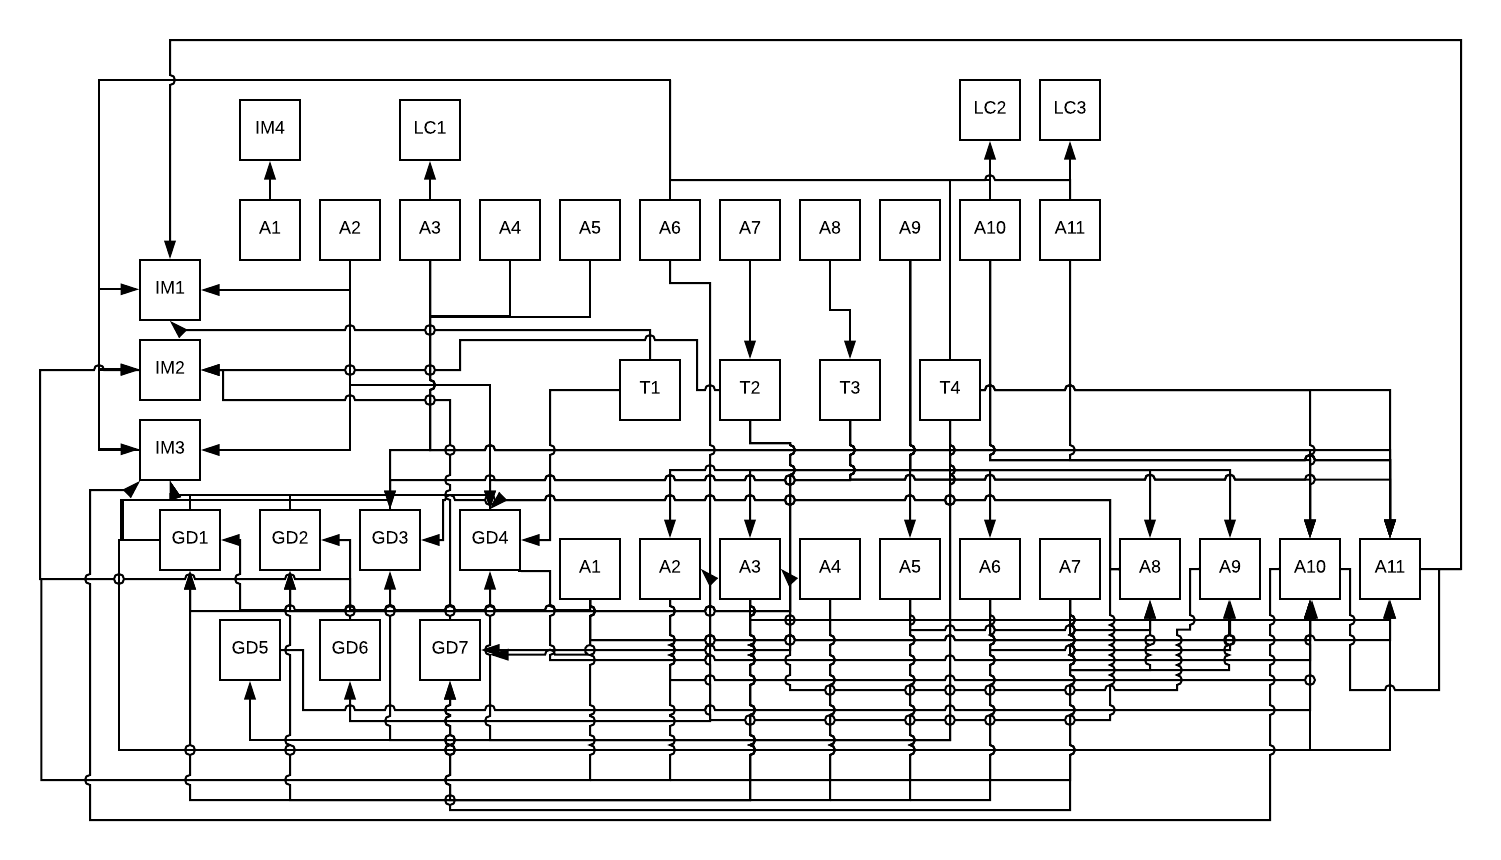
\includegraphics[width=\textwidth]{ATrace.png}
		}
		\caption{\label{Fig_ATrace} Traceability Matrix Showing the Connections 
		Between Items of Different Sections}
	\end{center}
\end{figure}


\begin{figure}[h!]
	\begin{center}
		%\rotatebox{-90}
		{
			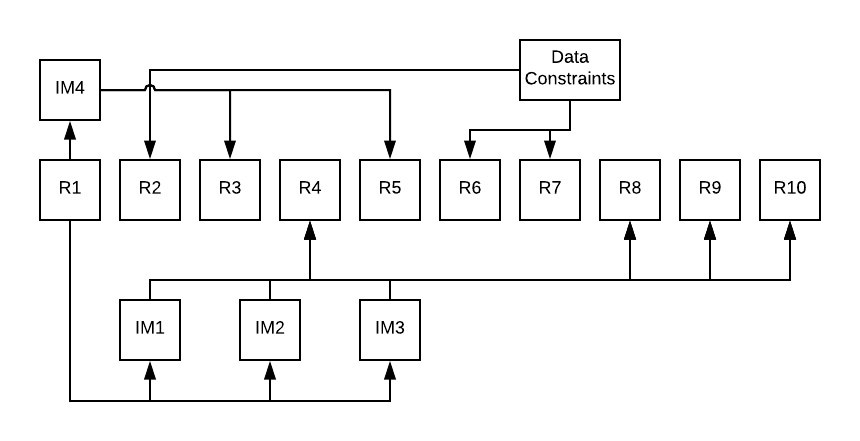
\includegraphics[width=0.7\textwidth]{RTrace.png}
		}
		\caption{\label{Fig_RTrace} Traceability Matrix Showing the Connections 
		Between Requirements, Instance Models, and Data Constraints}
	\end{center}
\end{figure}

\newpage

\bibliographystyle {plainnat}
\bibliography {../../refs/References}

\section{Appendix}

\subsection{Symbolic Parameters}
There are no symbolic parameters.

\end{document}
